\section{Auswertung}
\label{sec:Auswertung}

Die Versuche wurden aus Zeitgründen nur mit dem Computer durchgeführt. Analysiert wurden die Ergebnisse mittels Matplotlib, NumPy, SciPy und Uncertainties.

\subsection{1D-Festkörper}

Die Peaks der Resonanzen sind für die Messungen für ein bis zwölf Zylinder in Tabelle \ref{tab:rohr} aufgetragen. 
Daraus lässt sich mit Formel \ref{eq:speed} die Schallgeschwindigkeit zu \SI{320}{\meter\per\second} bestimmen. 

Die Spektren für \num{1} bis \num{12} Zylinder sind in Abb. \ref{fig:spec12} aufgetragen.

\begin{figure}
    \centering
    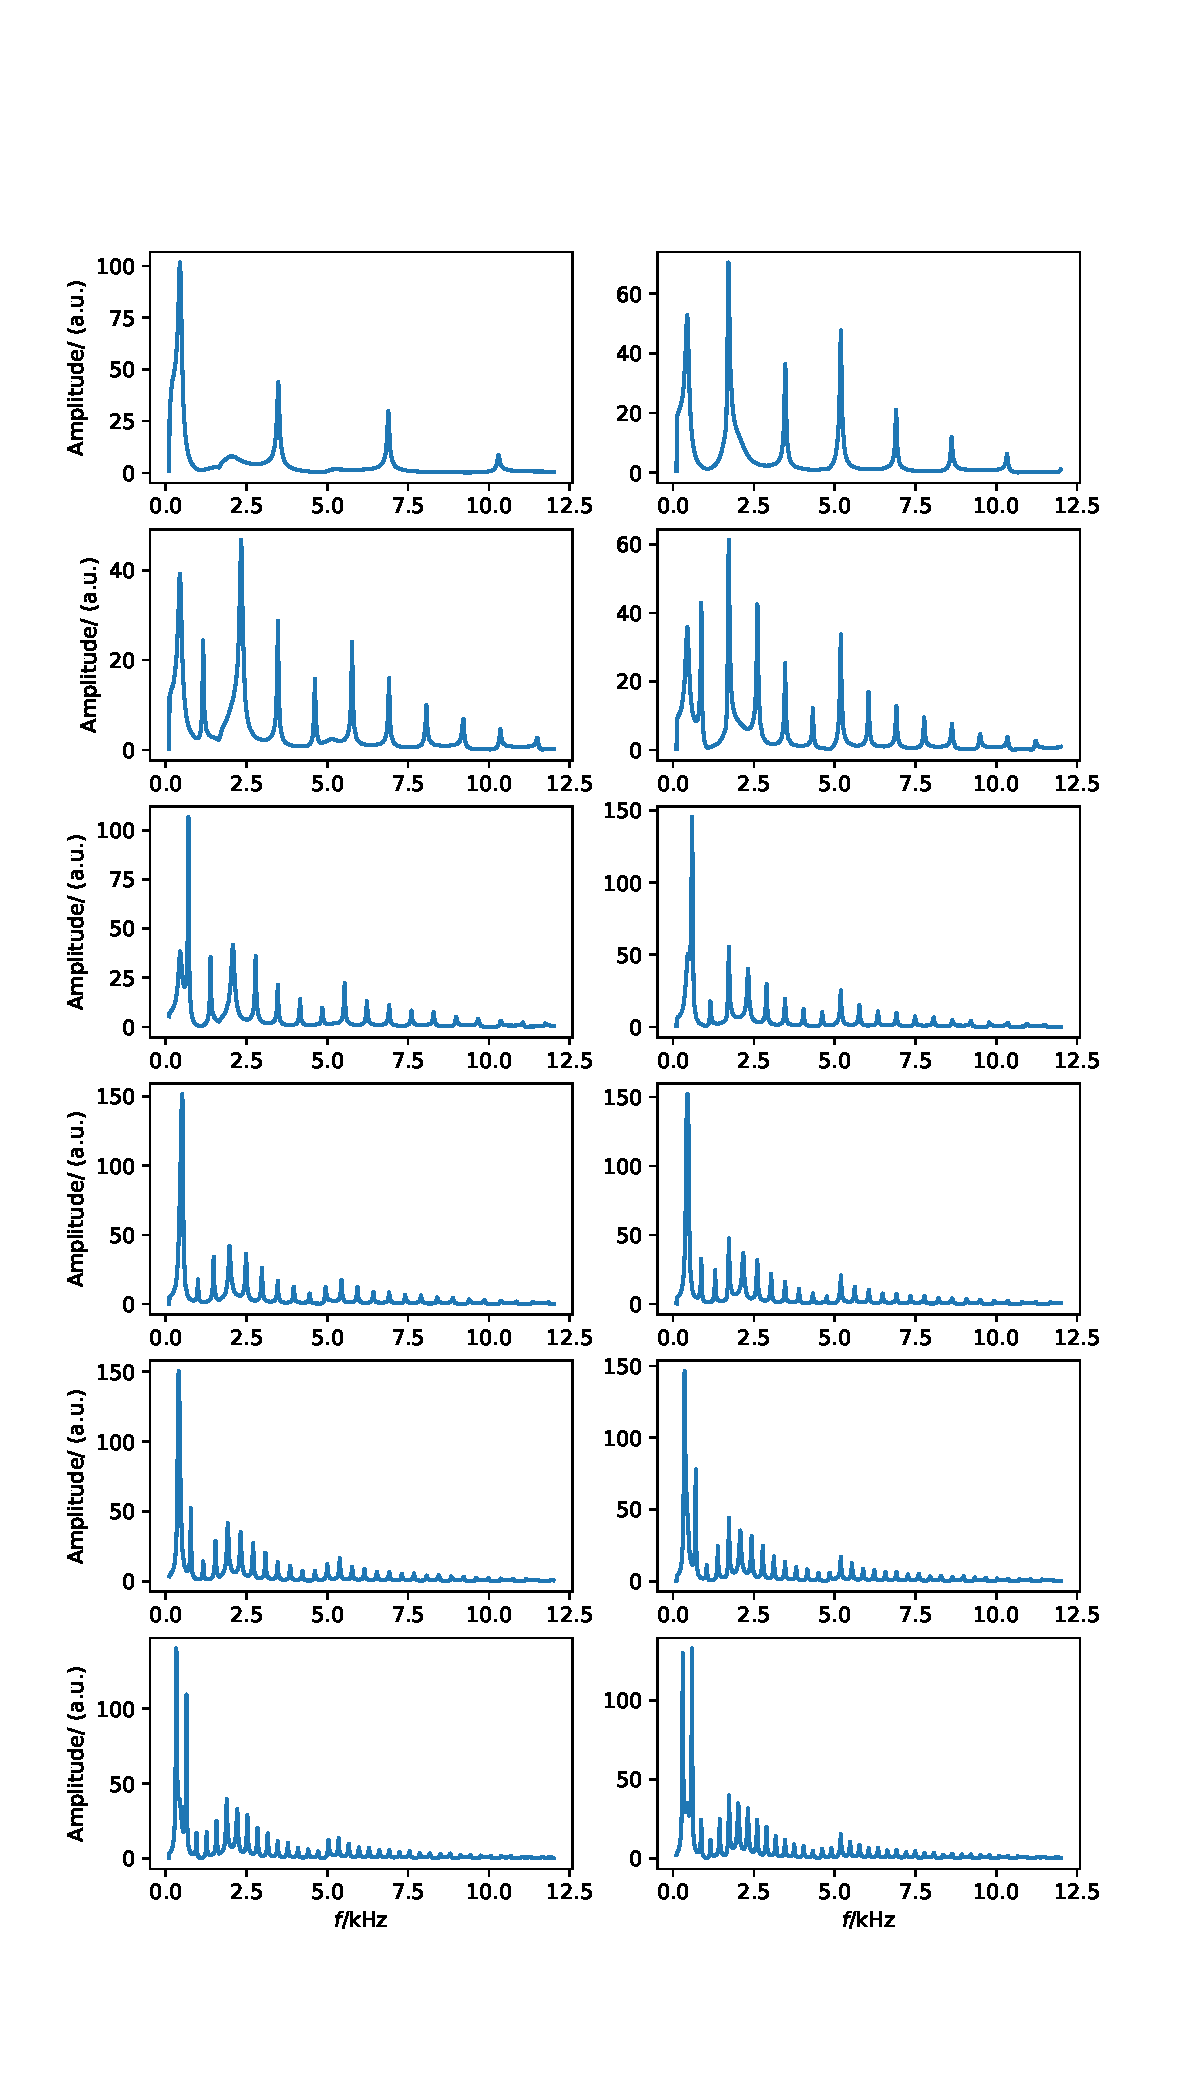
\includegraphics[width=0.8\textwidth]{plots/A_2.pdf}
    \caption{Das Frequenzspektrum für \num{1} (oben links) bis \num{12} Zylinder (unten rechts) mit jeweils einer Länge von \SI{50}{\milli\metre}.}
    \label{fig:spec12}
\end{figure}

Das Spektrum für einen einzelnen Zylinder der Länge $\SI{75}{\milli\metre}$ ist in Abb. \ref{fig:A3} zu sehen.
\begin{figure}
    \centering
    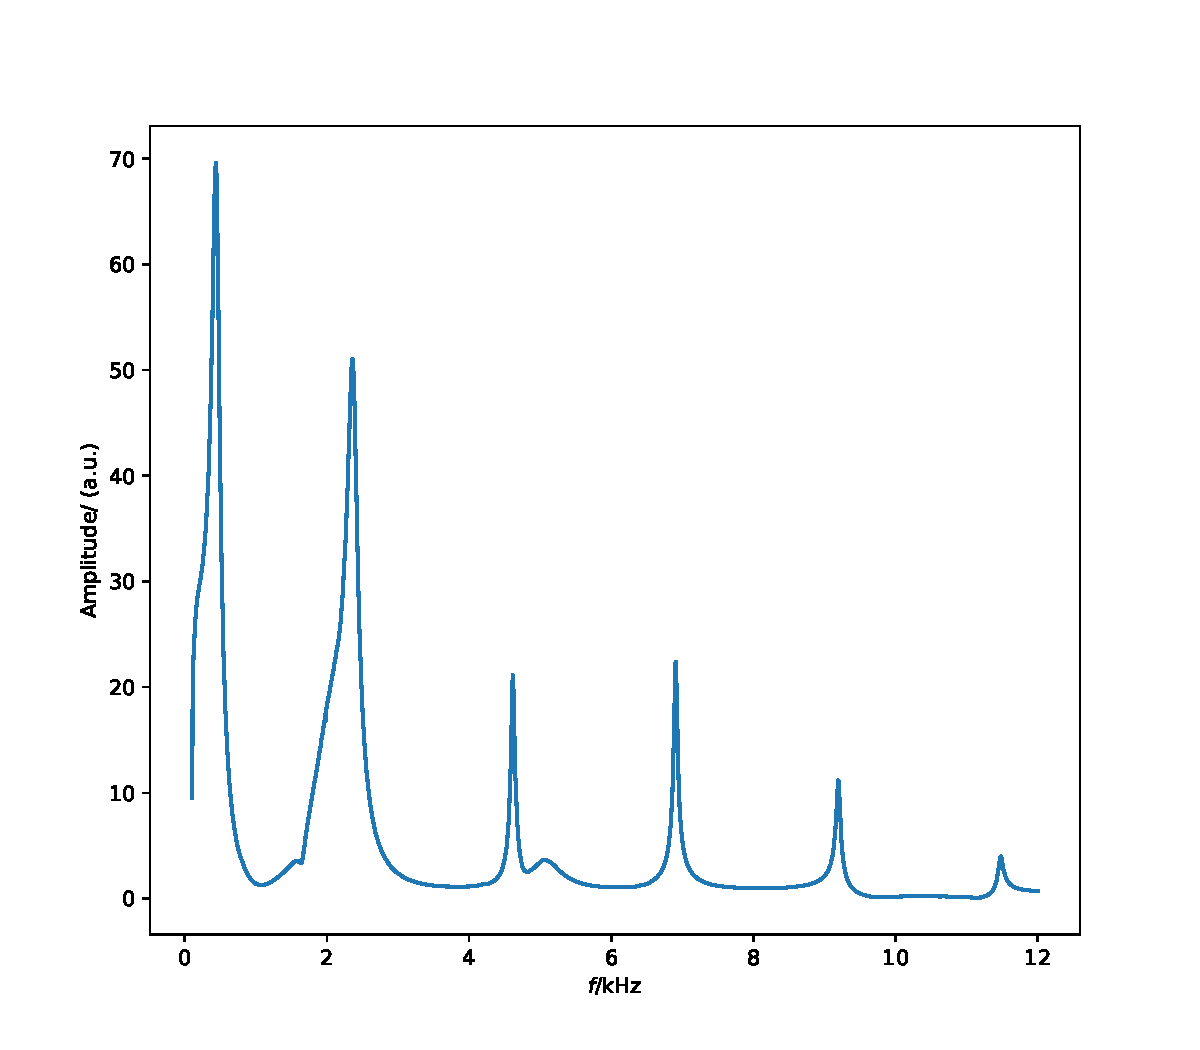
\includegraphics[width=0.8\textwidth]{plots/A_3.pdf}
    \caption{Das Frequenzspektrum für einen Zylinder mit einer Länge von \SI{75}{\milli\metre}.}
    \label{fig:A3}
\end{figure}

Für den größeren Zylinder ergibt sich analog eine Schallgeschwindigkeit von \SI{320}{\meter\per\second}.

Für jedes Rohr mit einer Blende kommt ein zusätzlicher Peak hinzu. 
Das Spektrum für \num{2} bis \num{10} Zylinder mit jeweils einer Blende dazwischen ist in Abb. \ref{fig:spec10} zu sehen. 

\begin{figure}
    \centering
    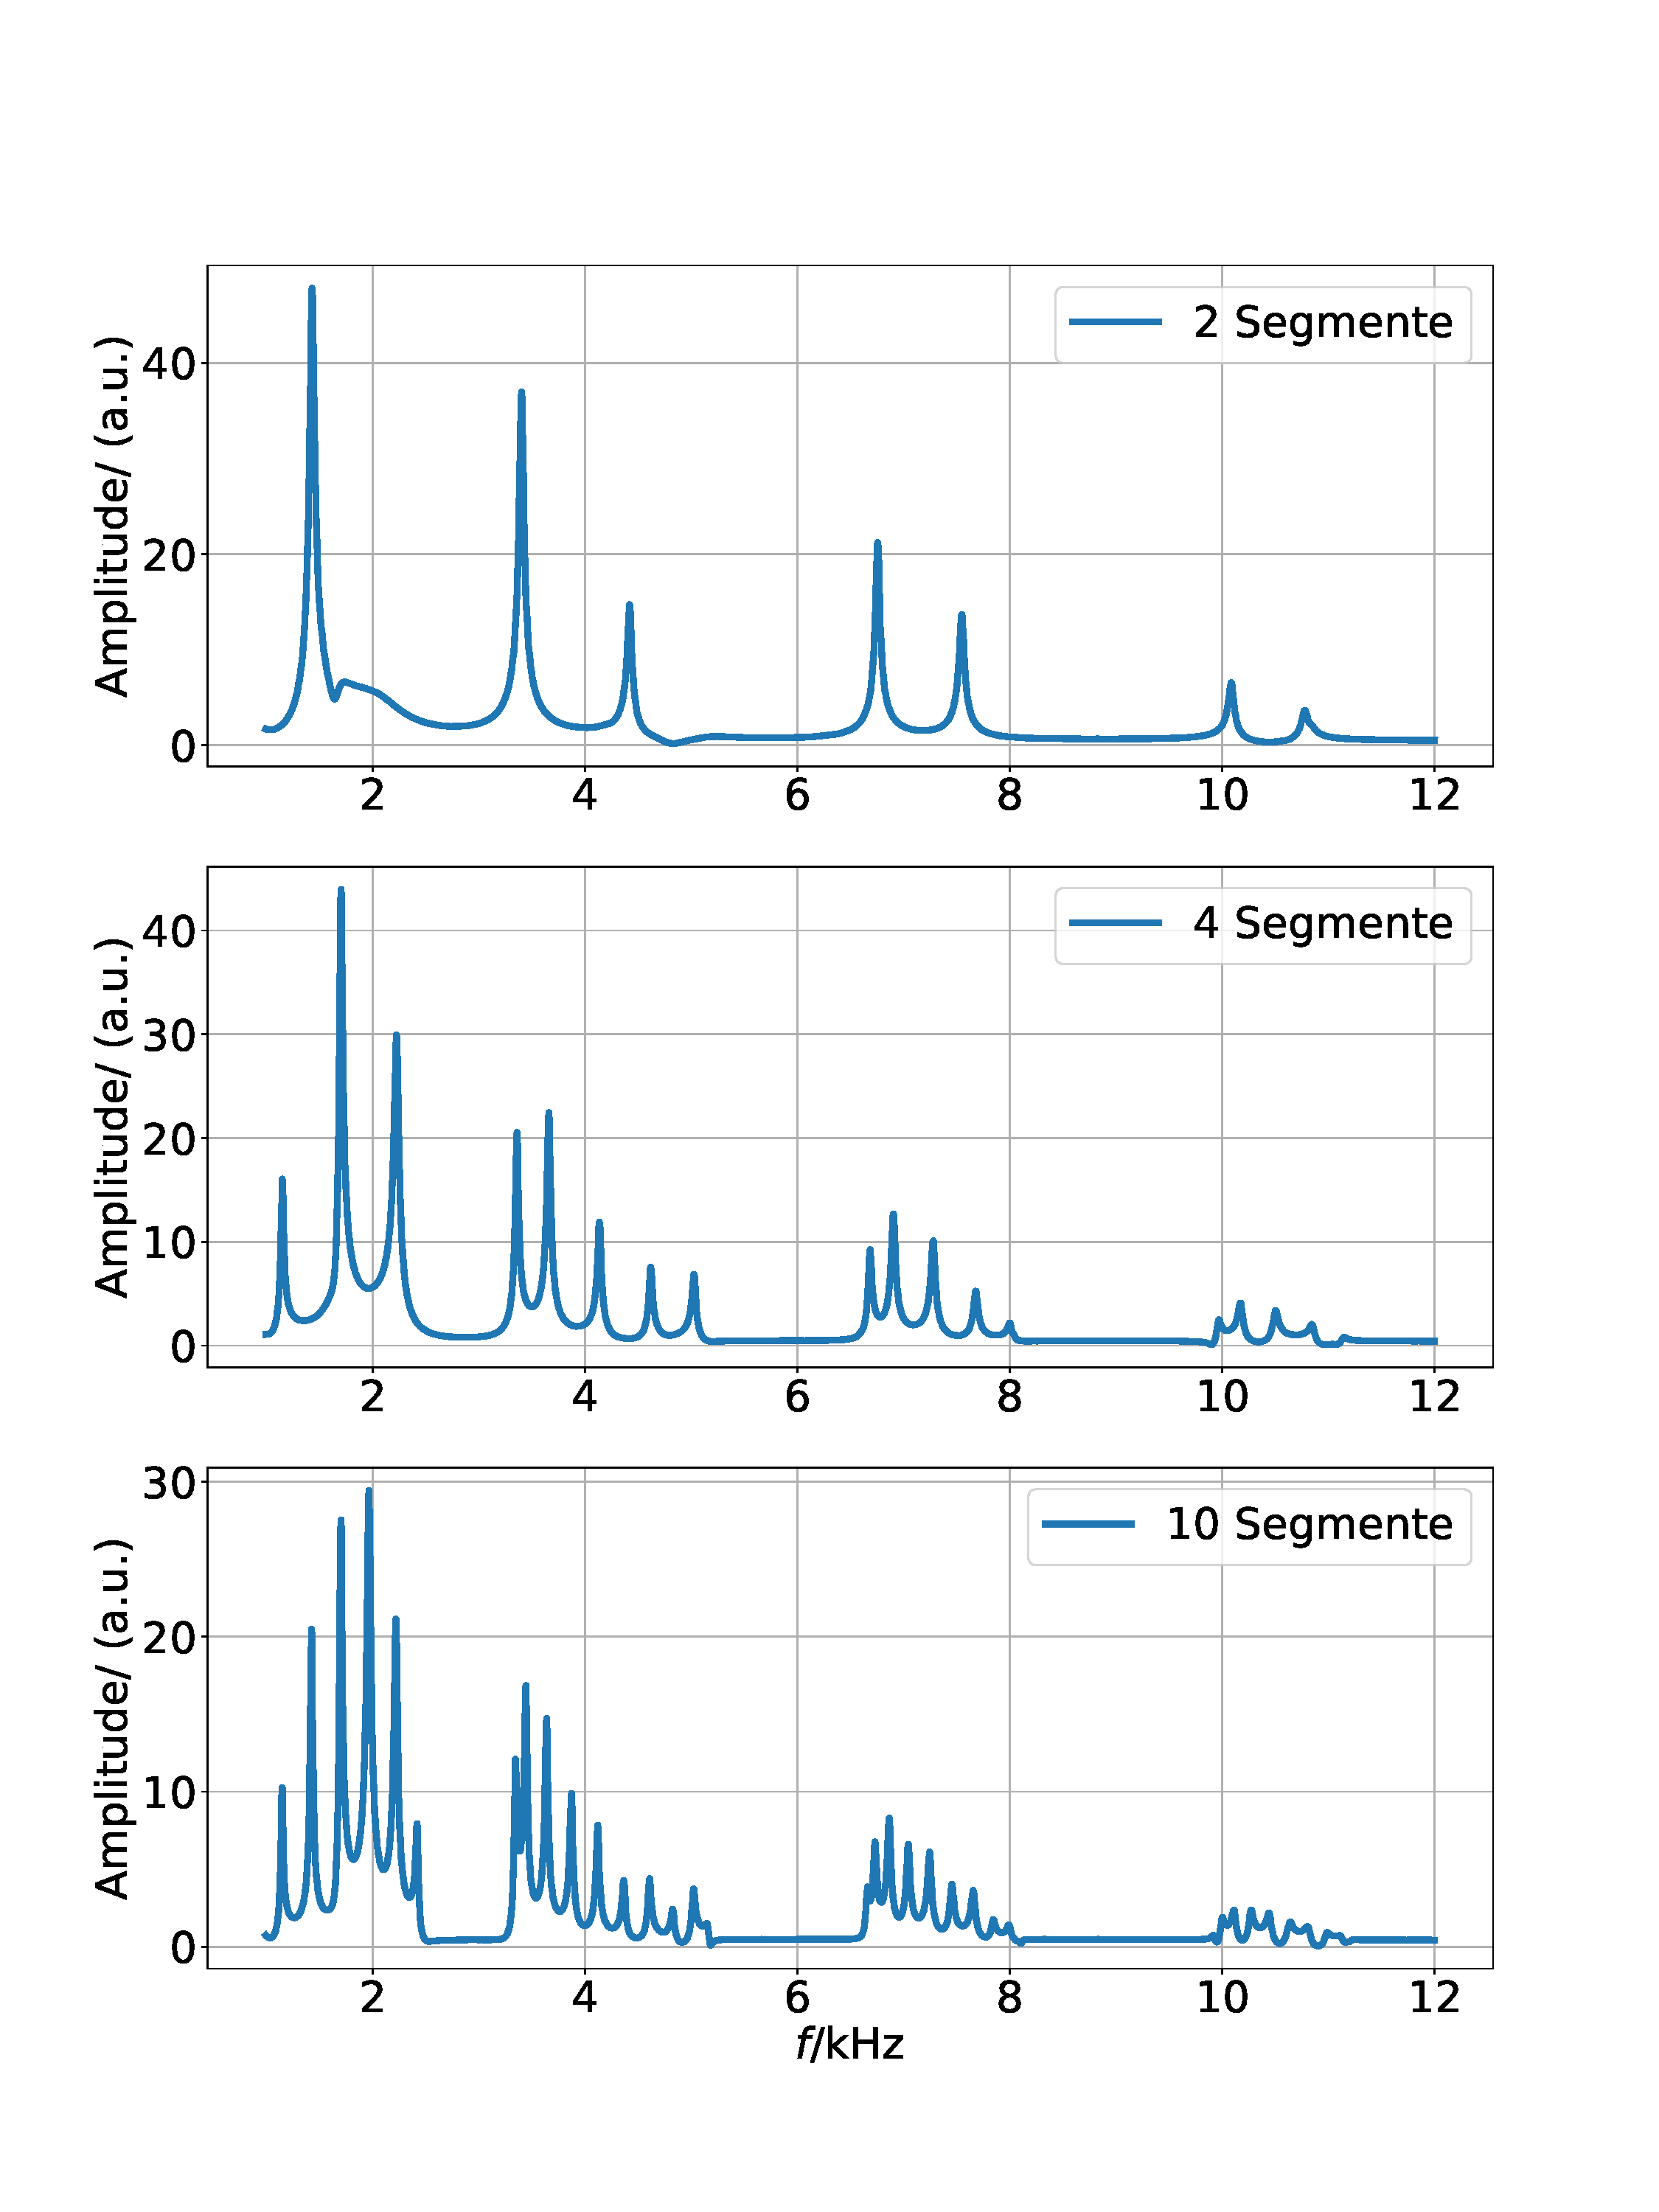
\includegraphics[width=0.8\textwidth]{plots/B_1.pdf}
    \caption{Das Frequenzspektrum für \num{2} (oben) bis \num{10} Zylinder (unten) mit jeweils einer Länge von \SI{50}{\milli\metre}. Zwischen den Zylindern befinden sich jeweils Blenden mit einem Durchmesser von \SI{16}{\milli\metre}.}
    \label{fig:spec10}
\end{figure}

Das Ganze wird erneut für \num{2}, \num{4} und \num{10} Zylinder mit Blenden des Durchmessers \SI{13}{\milli\meter} und \SI{10}{\milli\meter} durchgeführt. Die Spektren mit der Blende von \SI{13}{\milli\meter} ist in Abb. \ref{fig:spec10_13} zu sehen, die mit der \SI{10}{\milli\meter} Blende in Abb. \ref{fig:spec10_10}. 

\begin{figure}
    \centering
    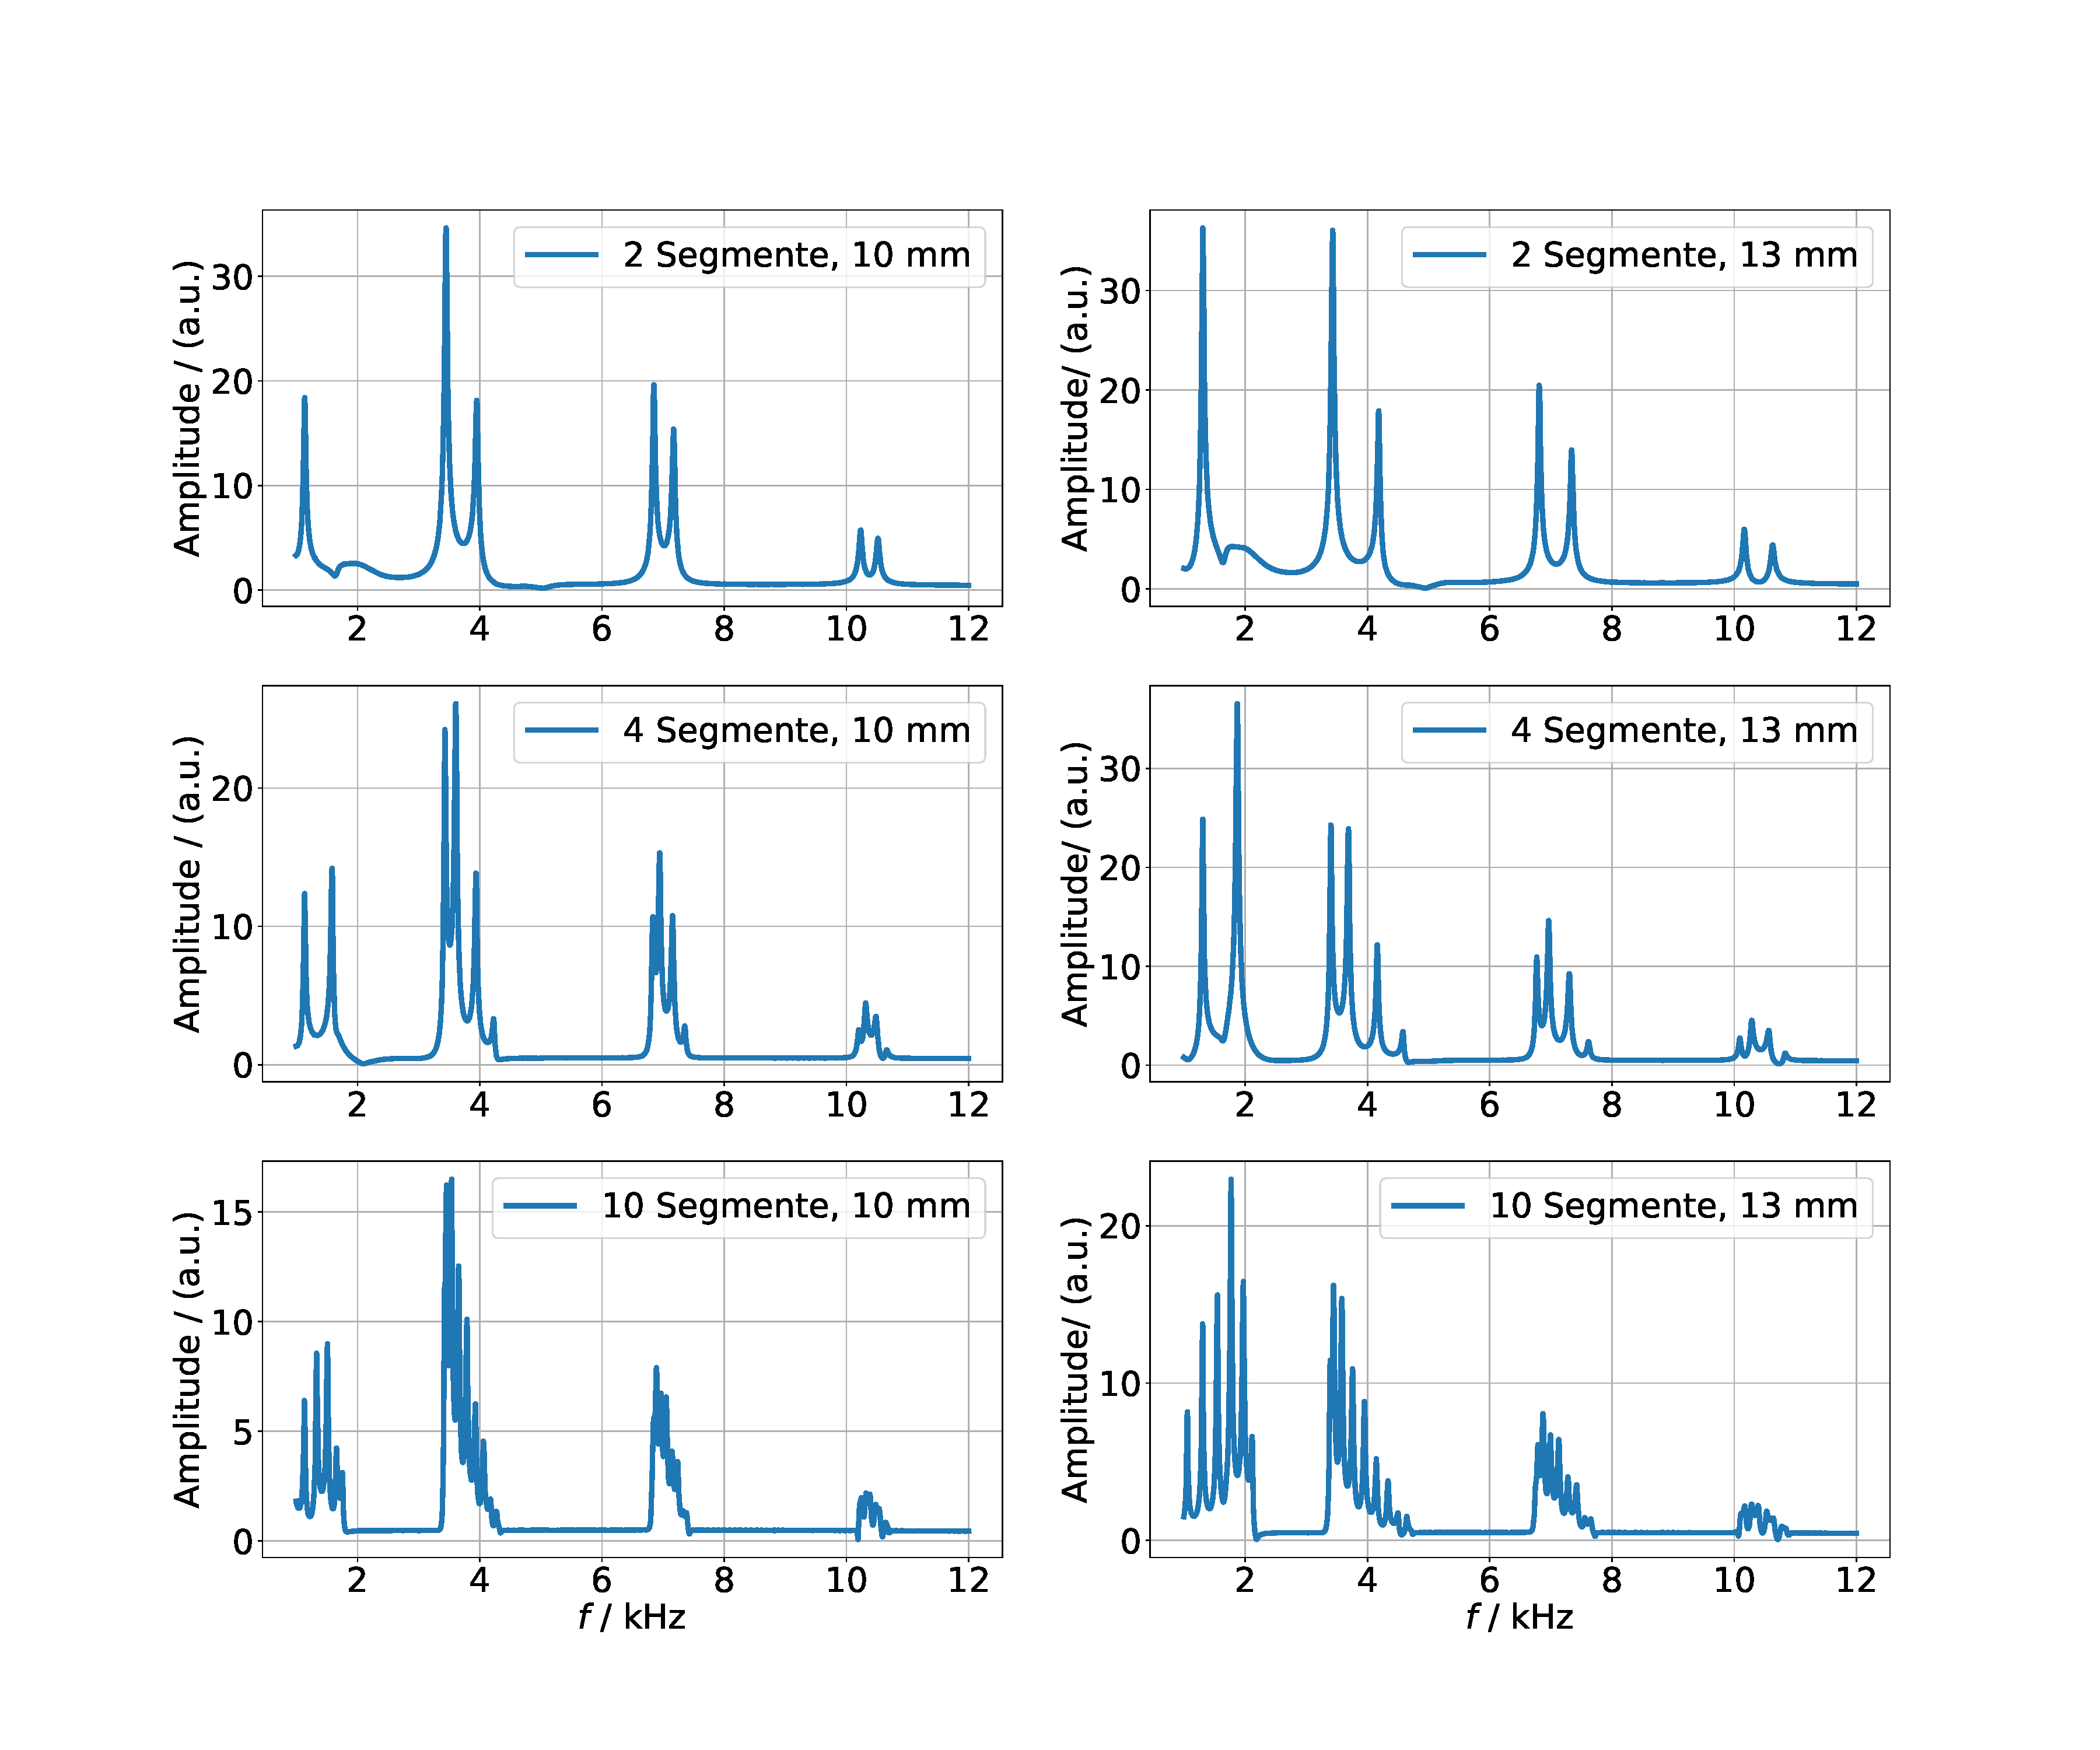
\includegraphics[width=0.8\textwidth]{plots/B_3.pdf}
    \caption{Das Frequenzspektrum für 10 Zylinder mit jeweils einer Länge von \SI{55}{\milli\metre} mit Blendendurchmesser von \SI{13}{\milli\metre}.}
    \label{fig:spec10_13}
\end{figure}

\begin{figure}
    \centering
    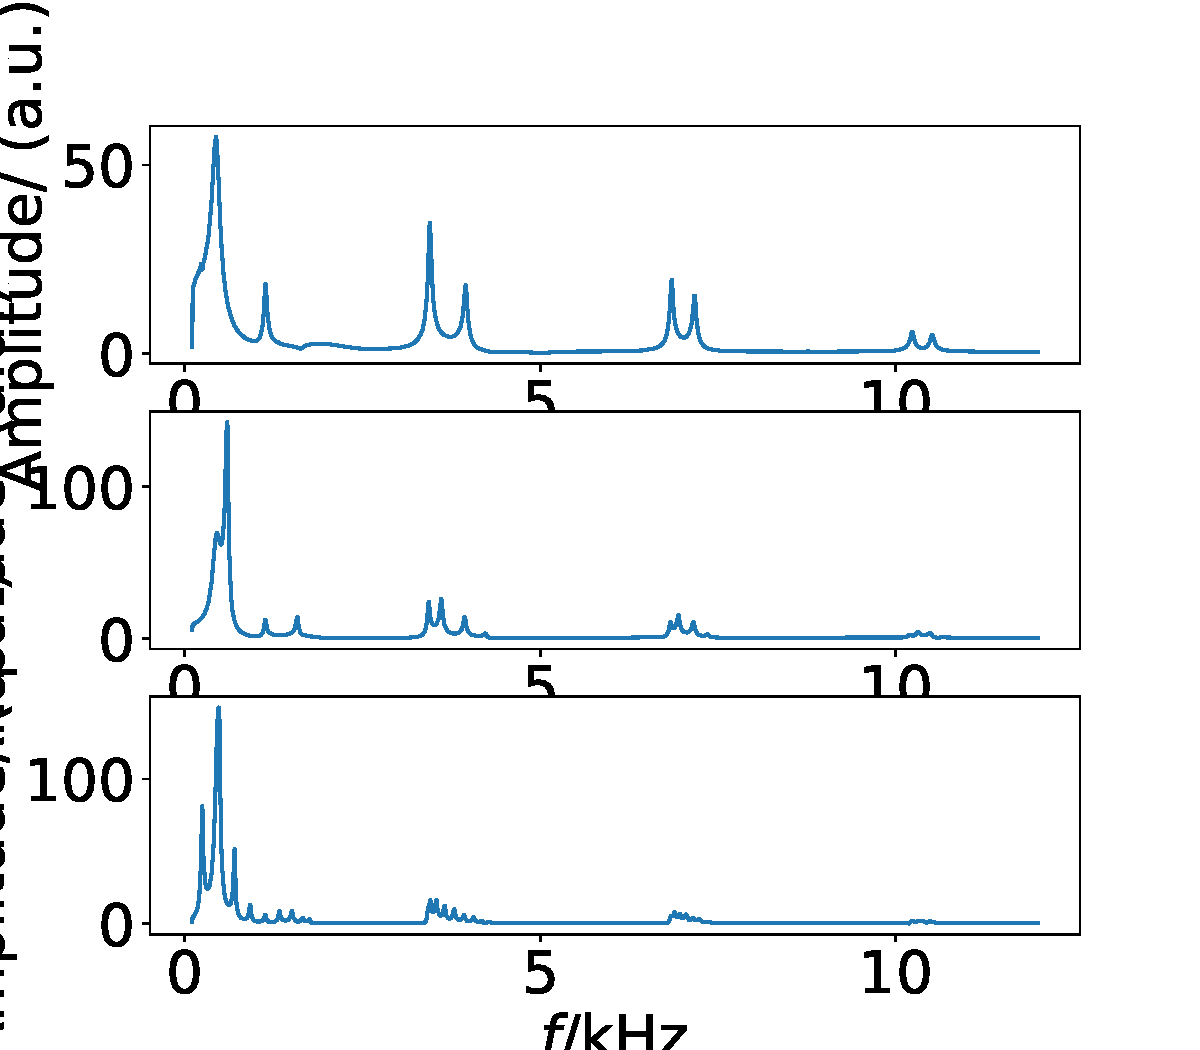
\includegraphics[width=0.8\textwidth]{plots/B_2.pdf}
    \caption{Das Frequenzspektrum für 10 Zylinder mit jeweils einer Länge von \SI{55}{\milli\metre} mit Blendendurchmesser von \SI{10}{\milli\metre}.}
    \label{fig:spec10_10}
\end{figure}

Die Messung wurde erneut variiert, indem einer der \num{10} Zylinder mit einer Länge von \SI{50}{\milli\meter} durch einen Zylinder anderer Länge ersetzt wurde. Die neuen Längen sind \SI{75}{\milli\meter}, \SI{37.5}{\milli\meter} und \SI{62.5}{\milli\meter}.
Die Veränderung ist in Abb. \ref{fig:var3} zu sehen.
\begin{figure}
    \centering
    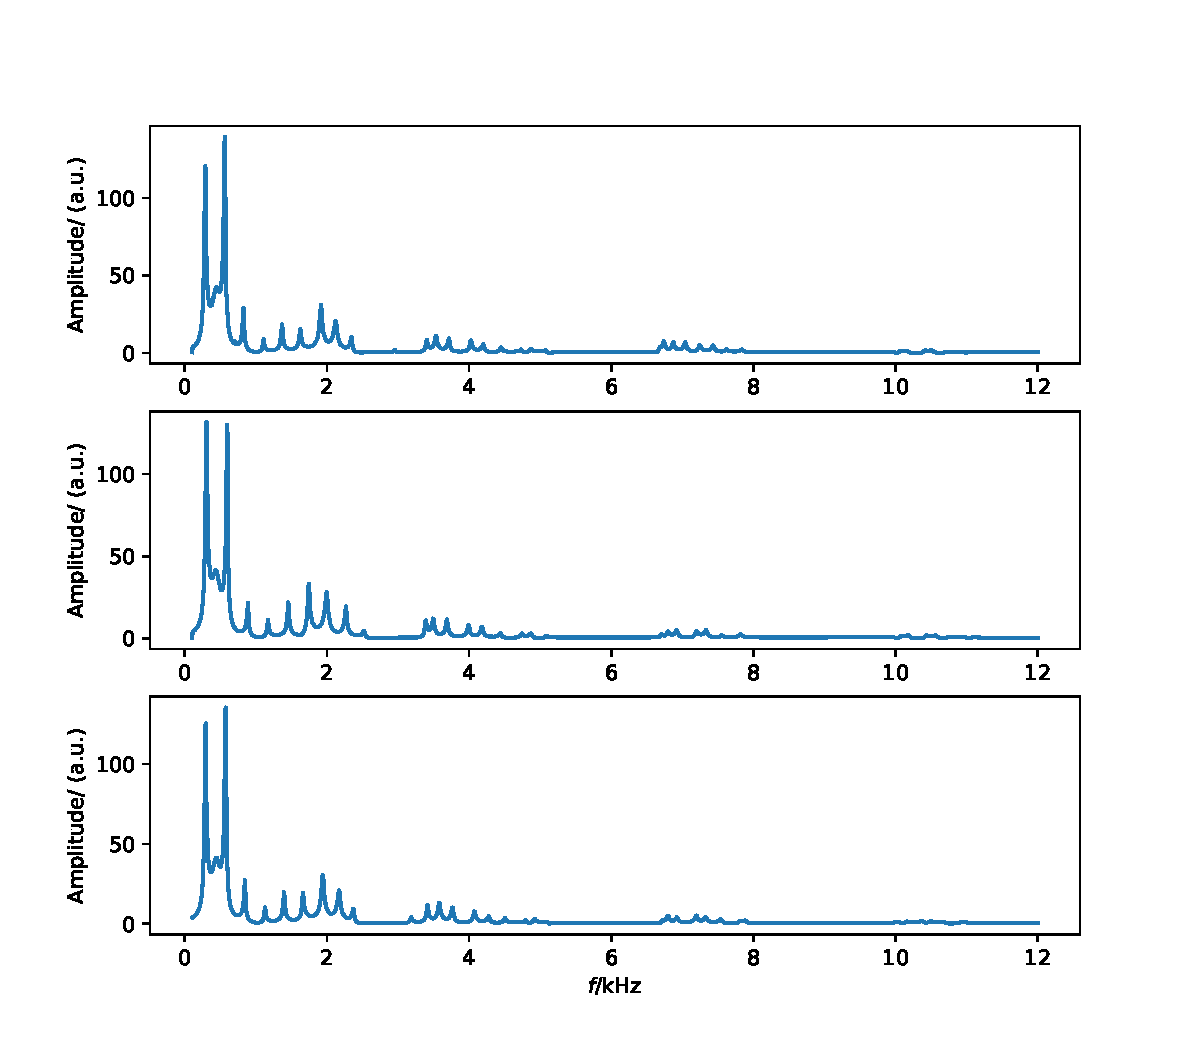
\includegraphics[width=0.8\textwidth]{plots/B_4.pdf}
    \caption{Das Frequenzspektrum für 9 Zylinder mit jeweils einer Länge von \SI{50}{\milli\metre} und einem Zylinder der Länge \SI{75}{\milli\metre} (oben), \SI{37.5}{\milli\metre} (Mitte), \SI{62.5}{\milli\metre} (unten). Der Blendendurchmesser beträgt \SI{16}{\milli\metre}.}
    \label{fig:var3}
\end{figure}


Eine Kette aus 10 Zylindern wurde abwechselnd aus \SI{50}{\milli\meter} und \SI{75}{\milli\meter} Zylindern zusammengesetzt mit \SI{16}{\milli\meter} Blenden.

Das Ergebnis im Vergleich zu einzelnen Zylindern der Längen \SI{50}{\milli\metre} und \SI{75}{\milli\metre} ist in Abb. \ref{fig:var4} zu sehen. 
\begin{figure}
    \centering
    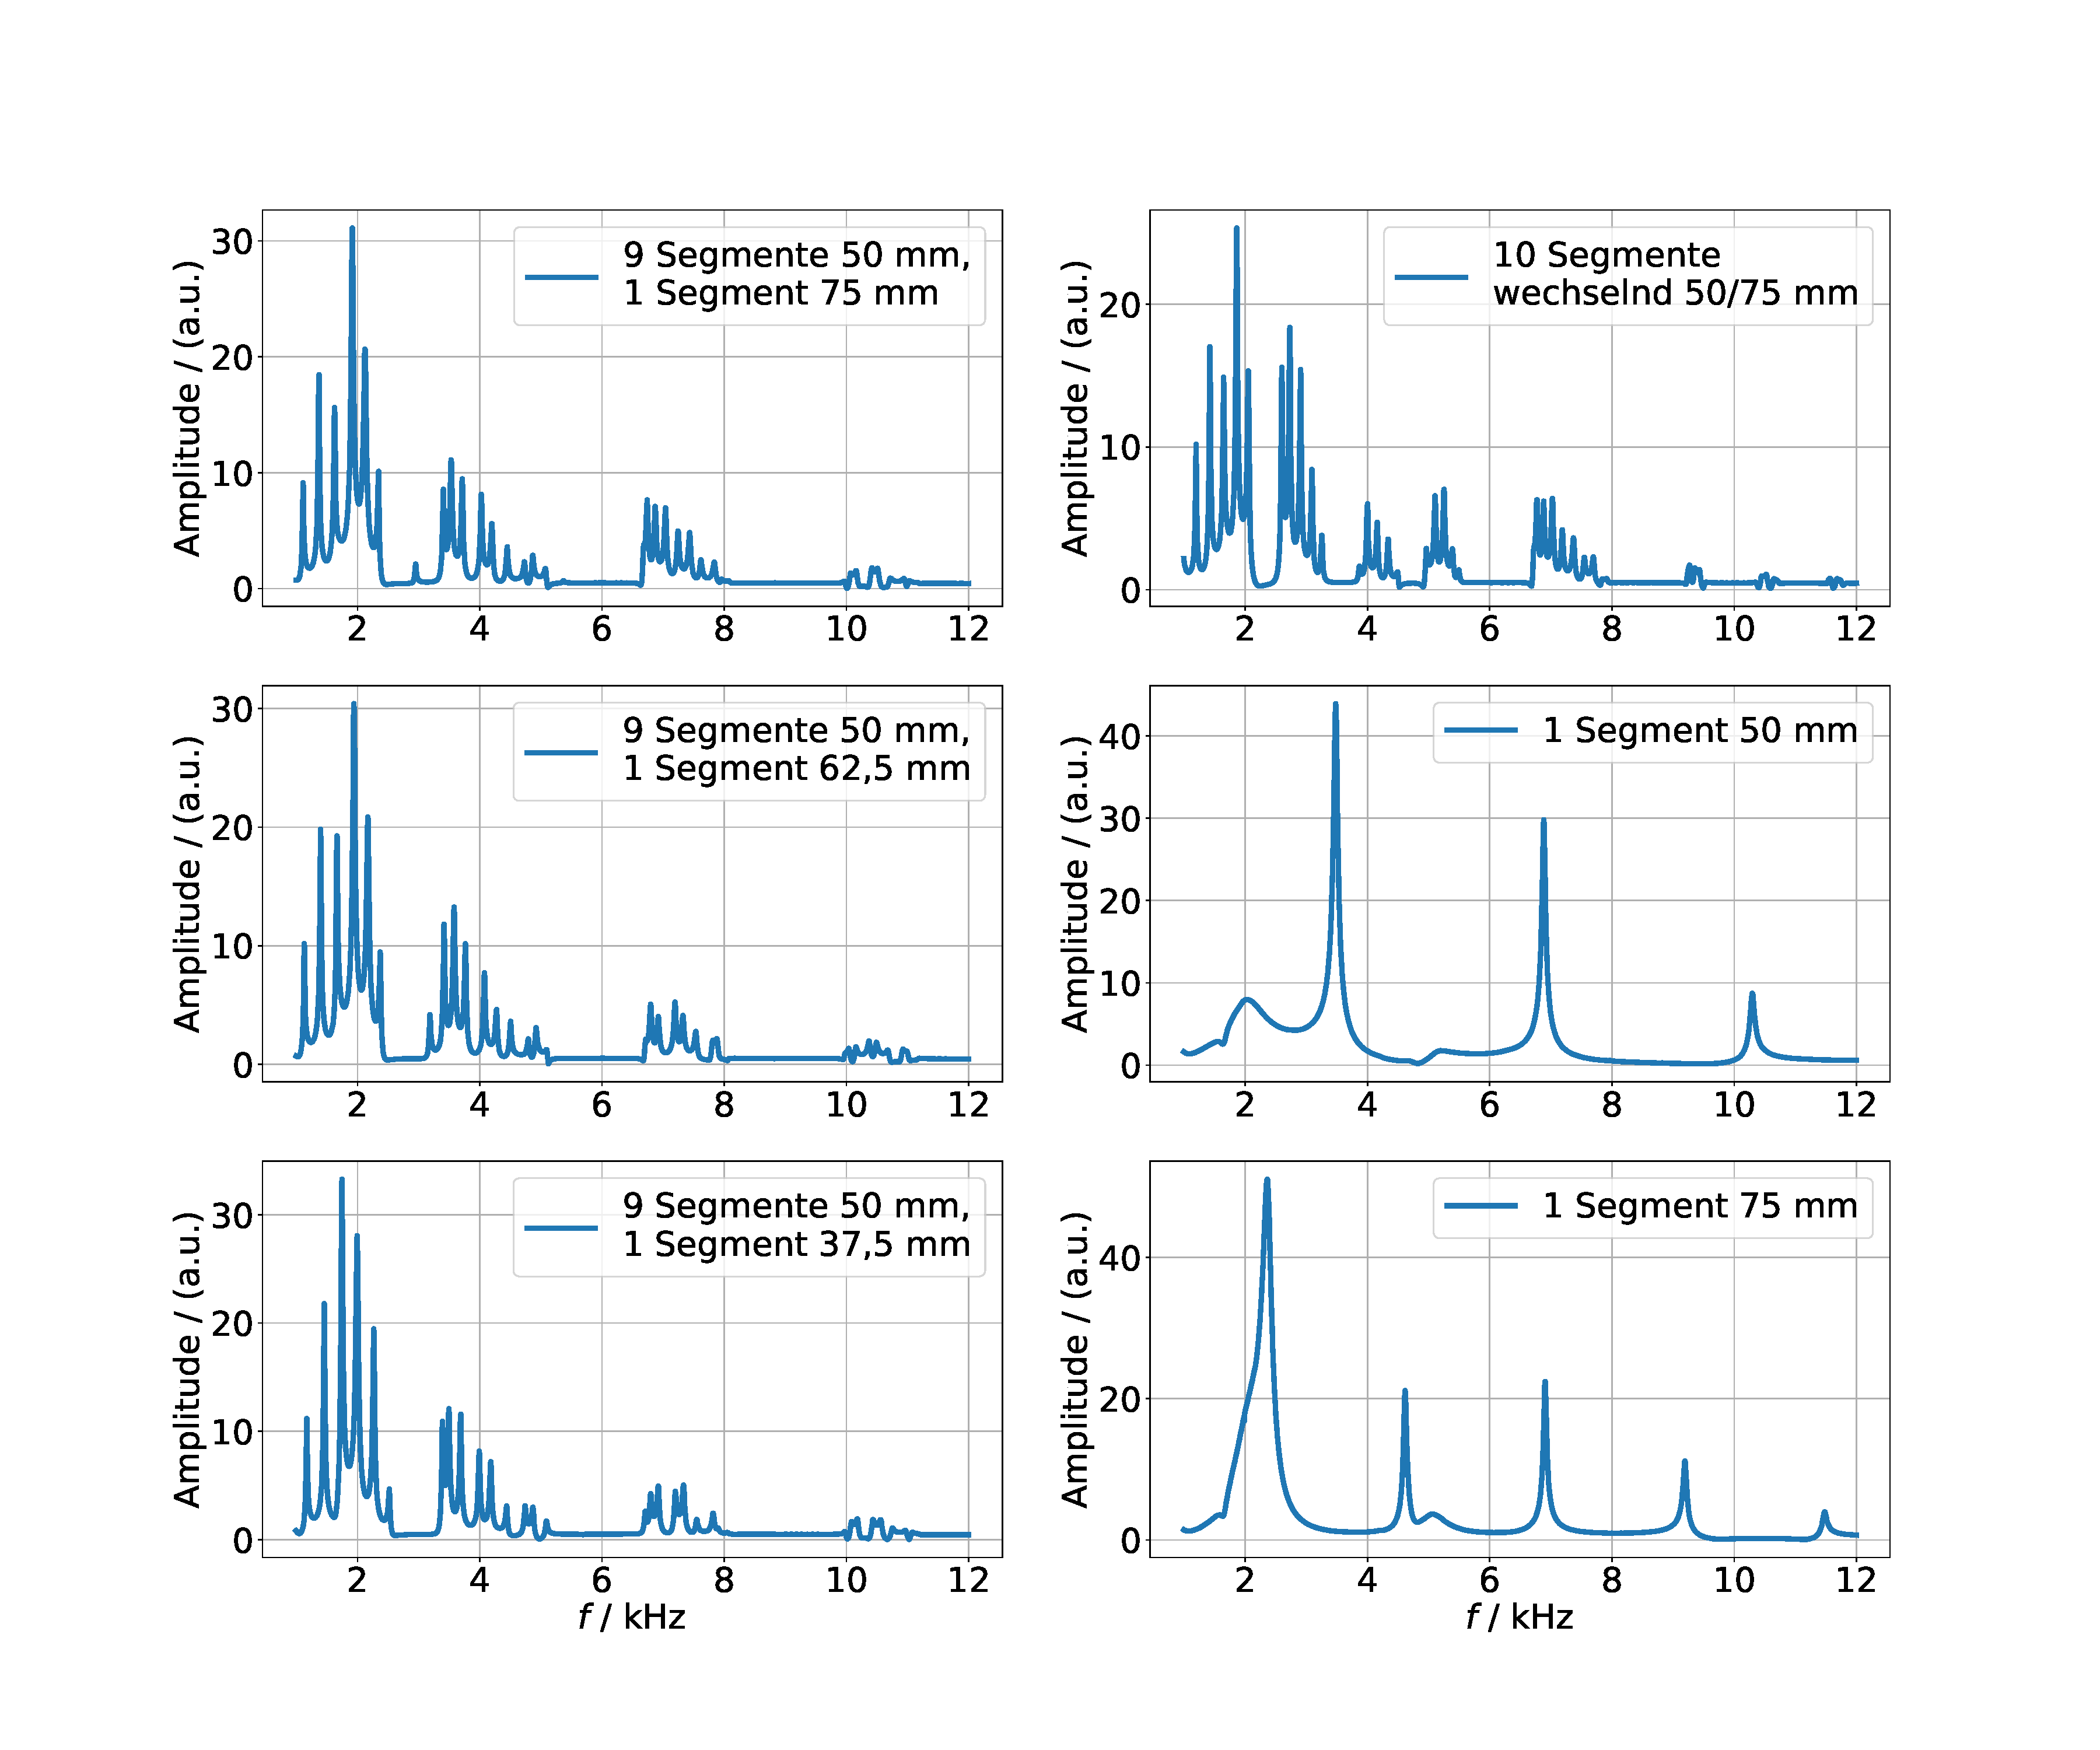
\includegraphics[width=0.8\textwidth]{plots/B_5.pdf}
    \caption{Oben ist das Frequenzspektrum einer Kette aus 10 Zylindern, deren Längen abwechselnd \SI{50}{\milli\metre} und \SI{75}{\milli\metre} betragen, zu sehen. Der Blendendurchmesser der zwischen den Zylindern platzierten Blenden beträgt \SI{16}{\milli\metre}. In der Mitte ist vergleichsweise das Frequenzspektrum für einen einzelnen Zylinder der Länge \SI{50}{\milli\metre} zu sehen, unten das für einen Zylinder der Länge \SI{75}{\milli\metre}.}
    \label{fig:var4}
\end{figure}

Die letzte Variation des Rohrresonators sind die \SI{13}{\milli\meter} und \SI{16}{\milli\meter} Blenden. Dafür wurden \num{8} Zylinder der Länge \SI{50}{\milli\metre} verwendet, zwischen die abwechselnd Blenden mit Durchmesser \SI{13}{\milli\metre} und \SI{16}{\milli\metre} gesetzt wurden. 

Die Ergebnisse sind in Abb. \ref{fig:var5} zu sehen.
\begin{figure}
    \centering
    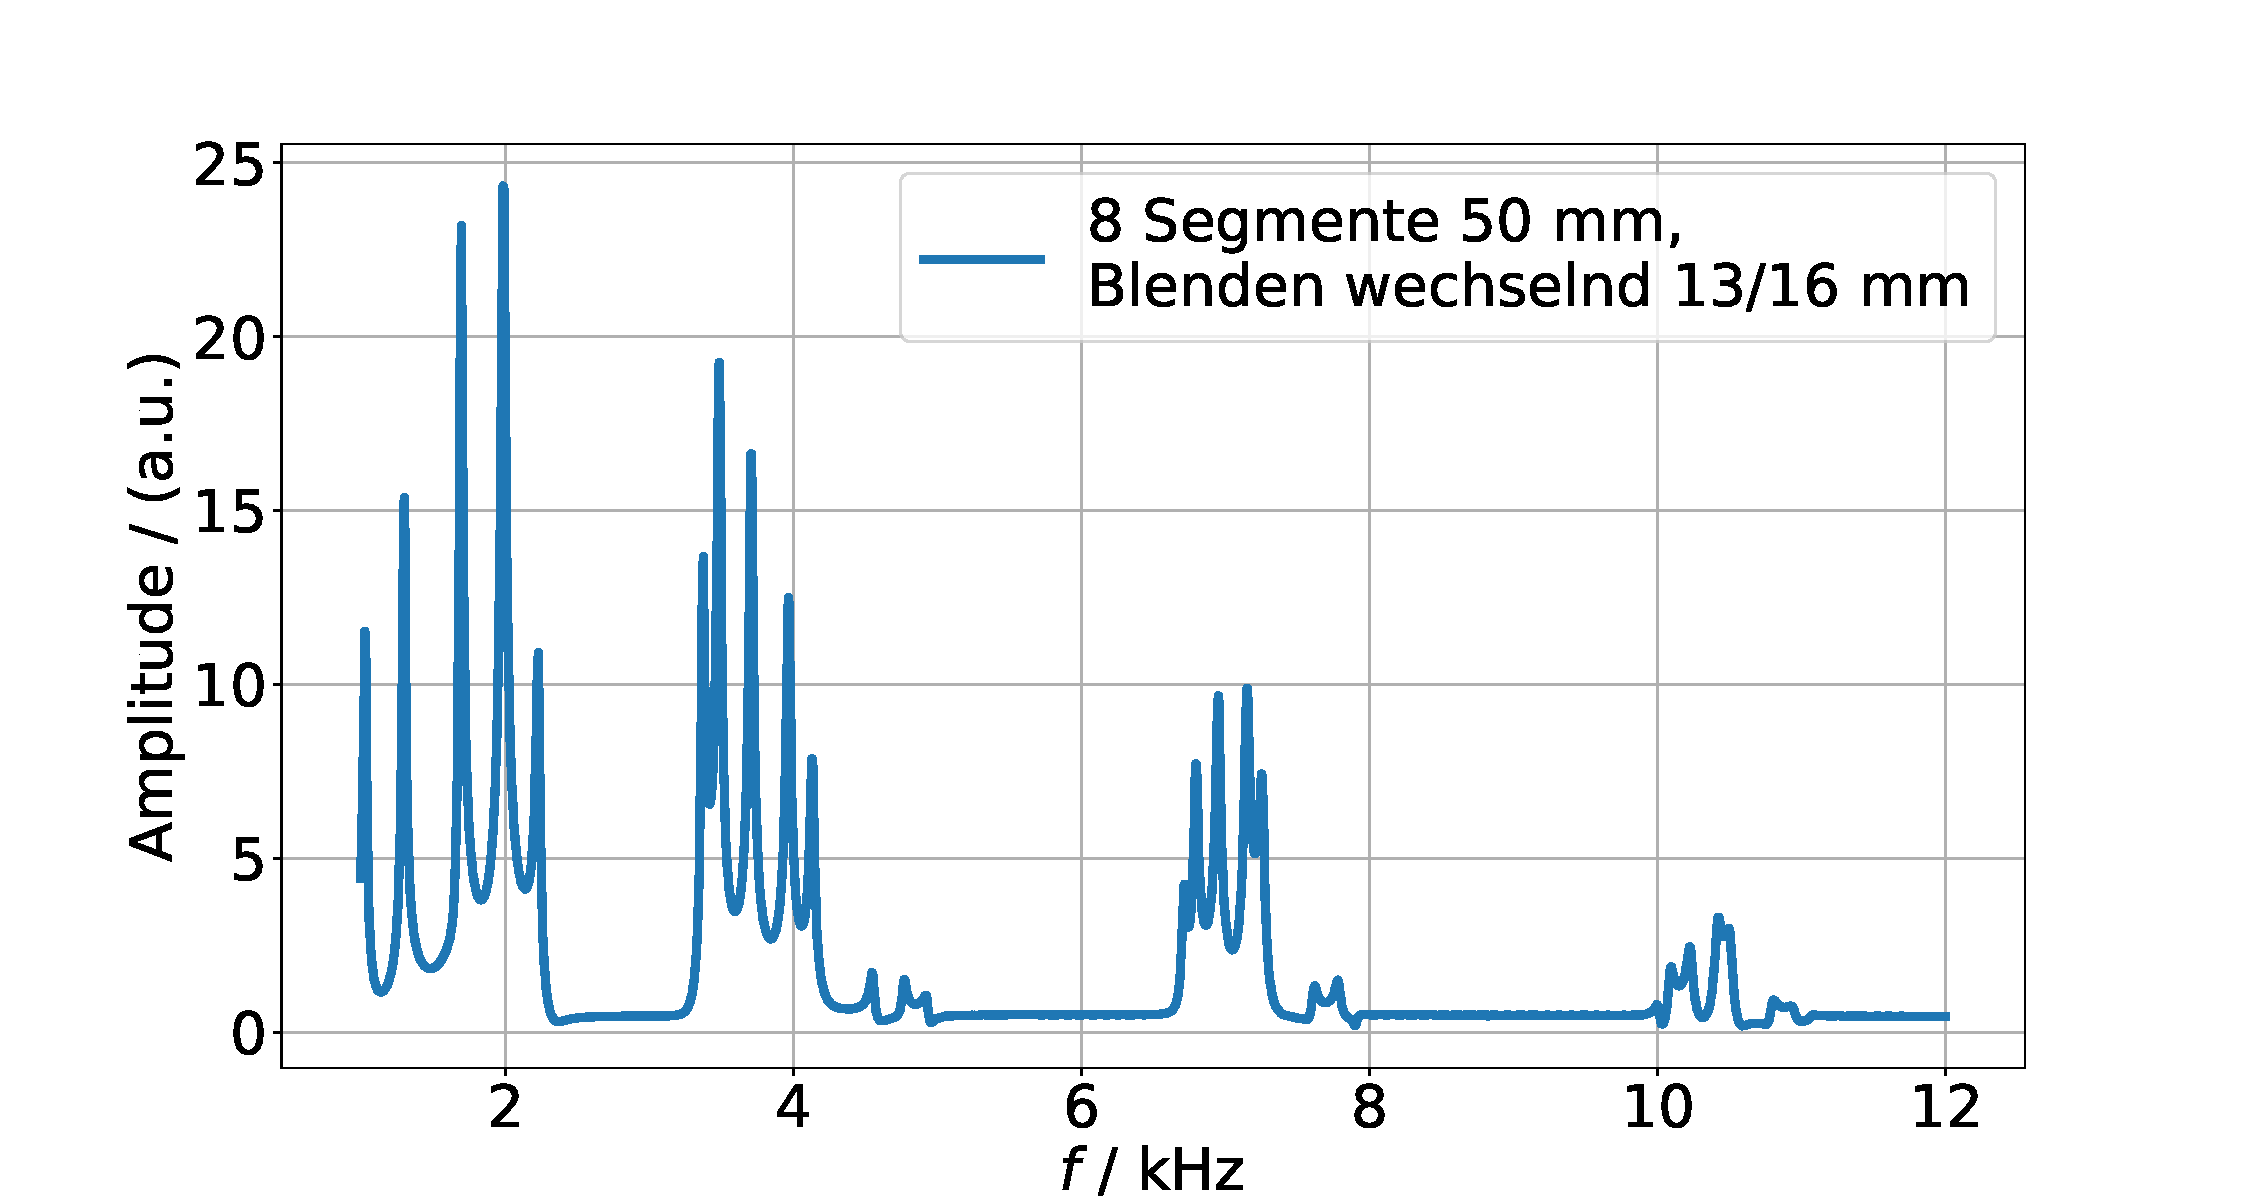
\includegraphics[width=0.8\textwidth]{plots/B_6.pdf}
    \caption{Das Frequenzspektrum für 8 Zylinder der Länge \SI{50}{\milli\metre}, zwischen die abwechselnd \SI{13}{\milli\metre} und \SI{16}{˜milli\metre} Blenden gesetzt wurden.}
    \label{fig:var5}
\end{figure}



\subsection{Wasserstoffatom}

In Abb. \ref{fig:Wasserstoff1} ist das Frequenzspektrum eines Kugelresonators bei einem Winkel von $\alpha = \SI{180}{\degree}$ zwischen Lautsprecher und Mikrofon zu sehen. %richtig?
Dabei werden Daten in \SI{5}{\hertz} Schritten bei \SI{60}{\milli\second} pro Schritt aufgenommen. %ist das wichtig?

\begin{figure}
    \centering
    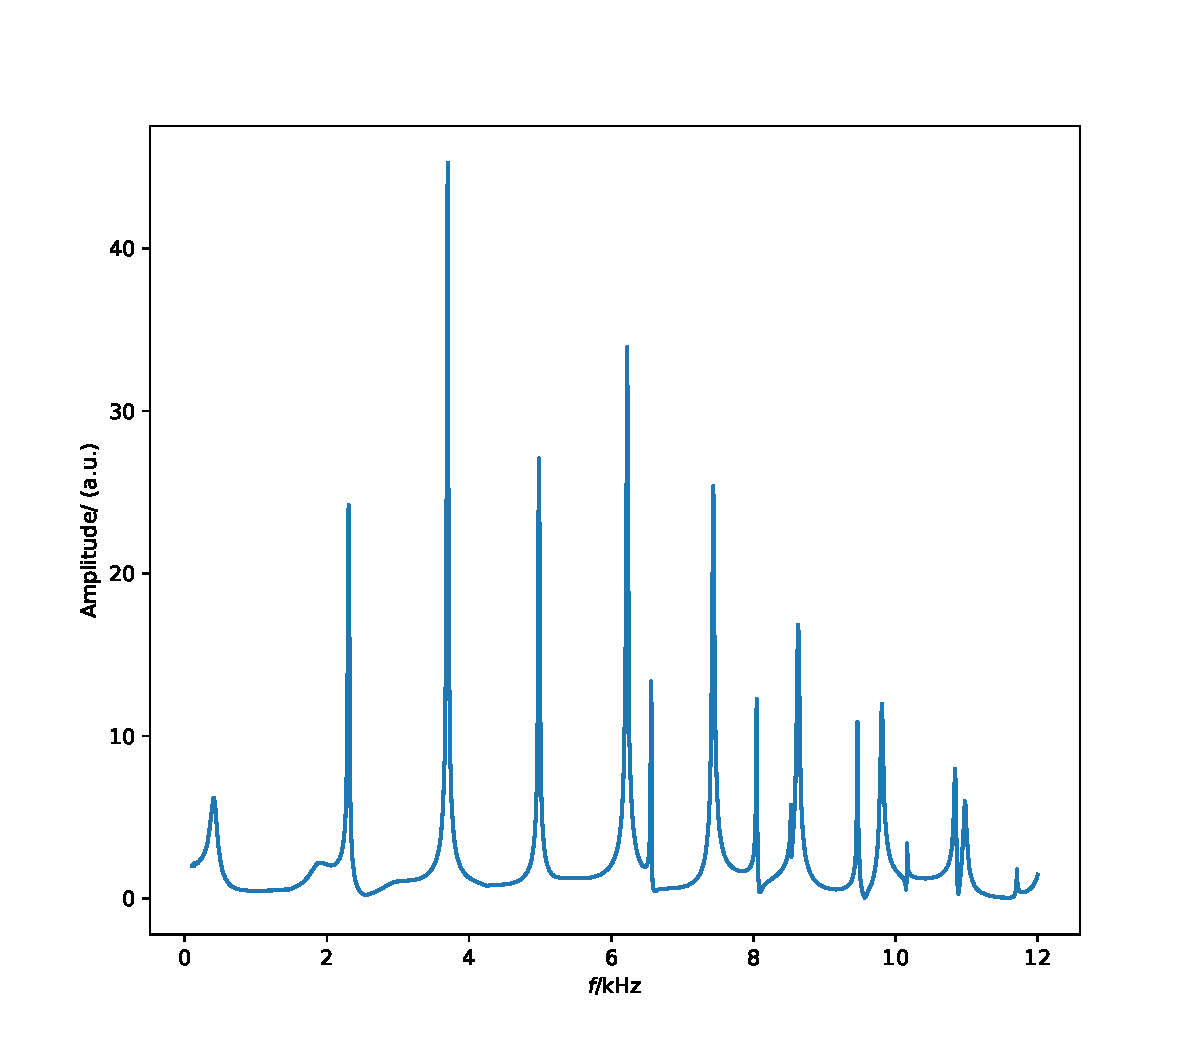
\includegraphics[width=0.8\textwidth]{plots/C_1.pdf}
    \caption{Zu sehen ist das Frequenzspektrum eines Kugelresonators bei einem eingestellten Winkel von \SI{180}{\degree}.}
    \label{fig:Wasserstoff1}
\end{figure}

Die Winkelabhängigkeit der Amplitude von den Resonanzen bei \SI{2.3}{\kilo\hertz}, \SI{3.7}{\kilo\hertz}, \SI{5}{\kilo\hertz} und bei \SI{7.4}{\kilo\hertz} wird im Folgenden untersucht. 

%In Tab. \ref{tab:winkelamp} sind die Amplitudenwerte für alle drei Peaks bei Winkeln von \SI{0}{\degree} bis \SI{180}{\degree} aufgetragen und in Abb. \ref{fig:Polar} als Polarplots abgebildet.
Dazu sind die Amplitudenwerte für alle vier Peaks bei Winkeln von \SI{0}{\degree} bis \SI{180}{\degree} in Polarplots abgebildet (Abb. \ref{fig:polar23}, \ref{fig:polar37}, \ref{fig:polar5}, \ref{fig:polar74}).


\begin{figure}
    \centering
    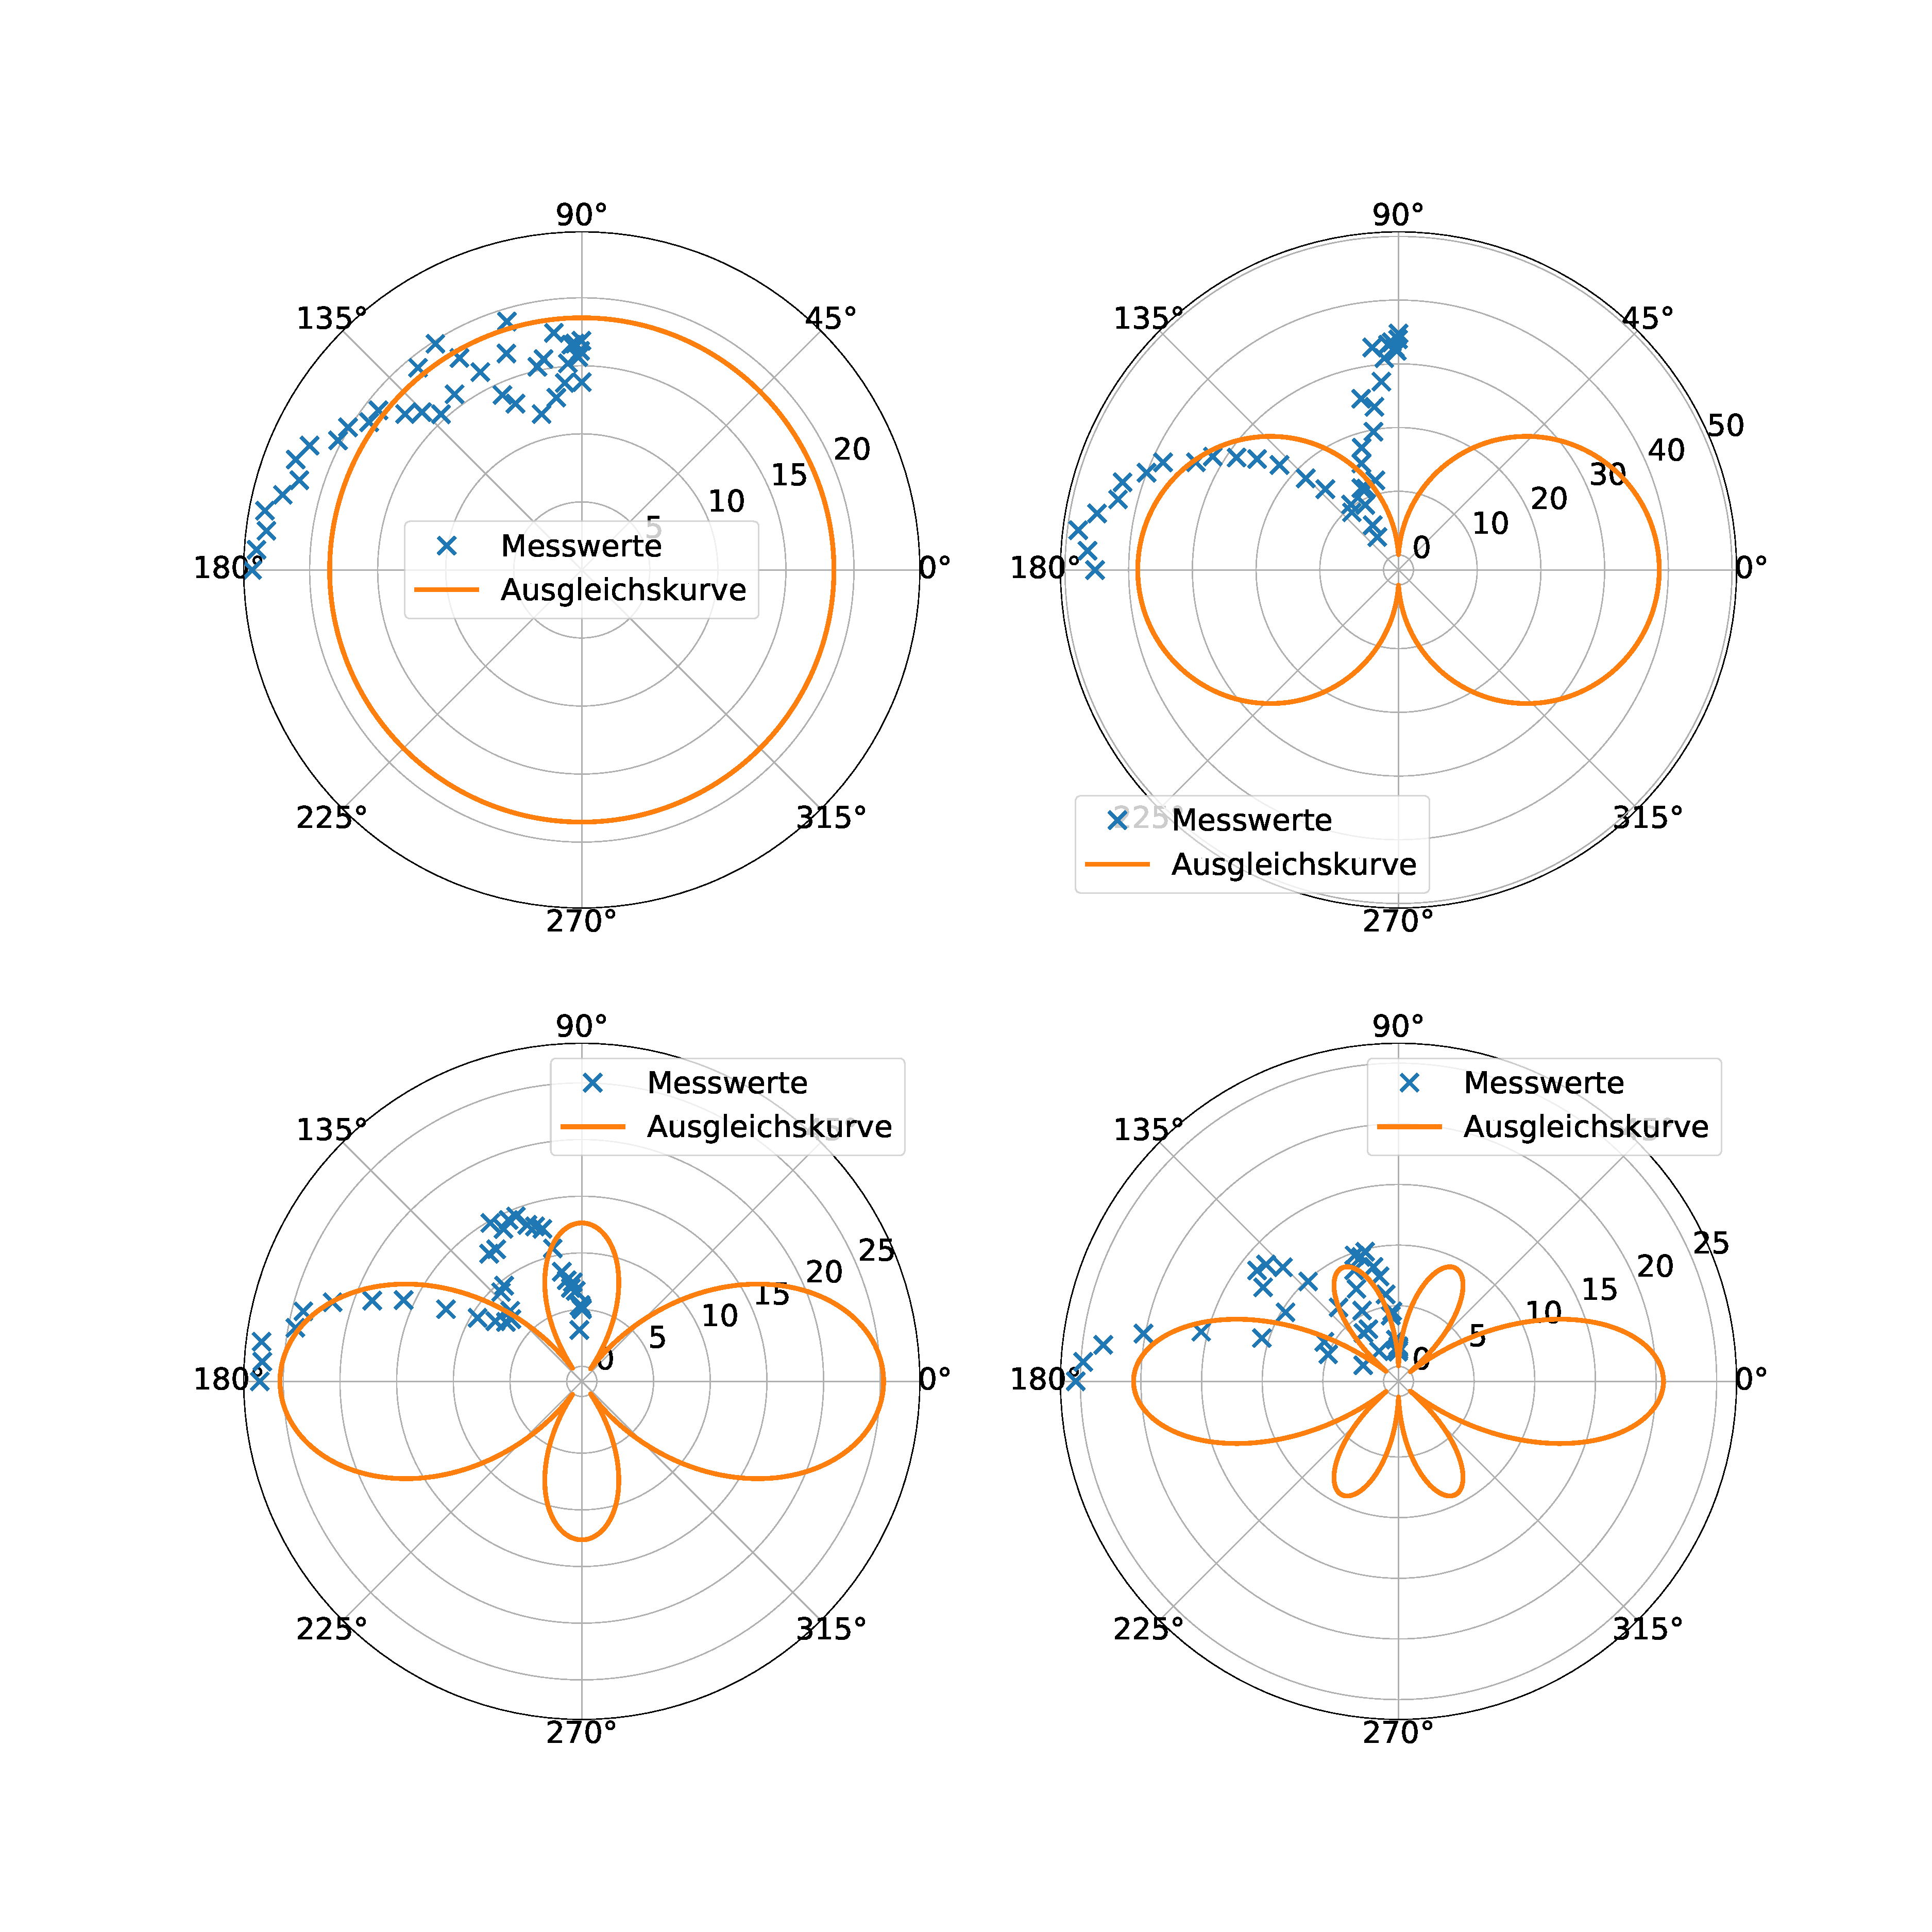
\includegraphics[width=0.8\textwidth]{plots/C_polar1.pdf}
    \caption{Die Winkelverteilung der Amplitude bei der Resonanzfrequenz von \SI{2.3}{\kilo\hertz}.}
    \label{fig:polar23}
\end{figure}

\begin{figure}
    \centering
    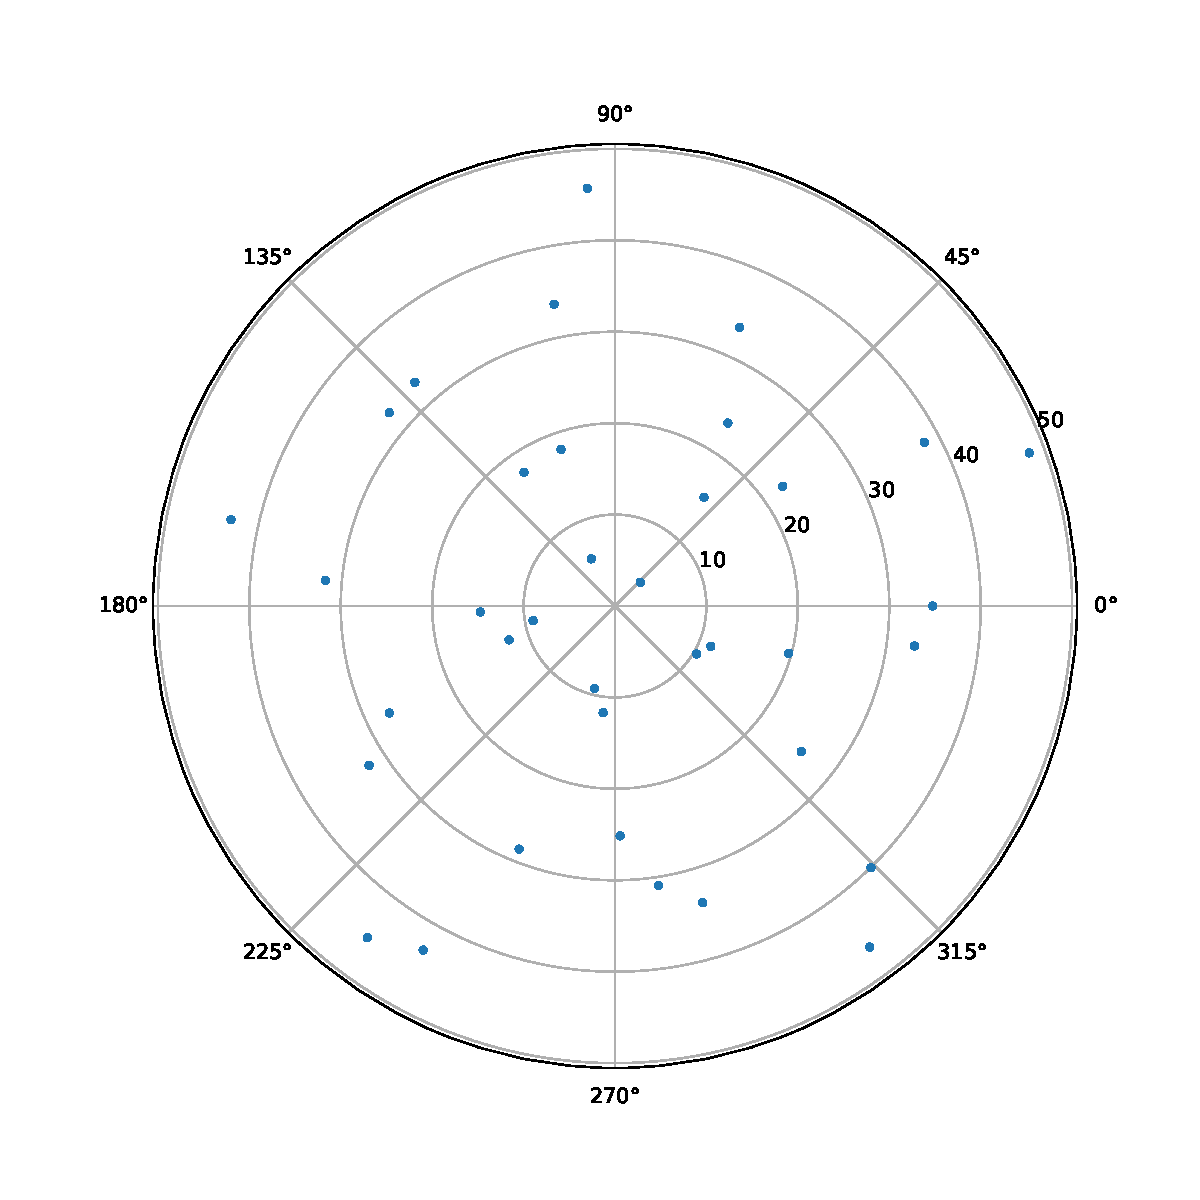
\includegraphics[width=0.8\textwidth]{plots/C_polar2.pdf}
    \caption{Die Winkelverteilung der Amplitude bei der Resonanzfrequenz von \SI{3.7}{\kilo\hertz}.}
    \label{fig:polar37}
\end{figure}

\begin{figure}
    \centering
    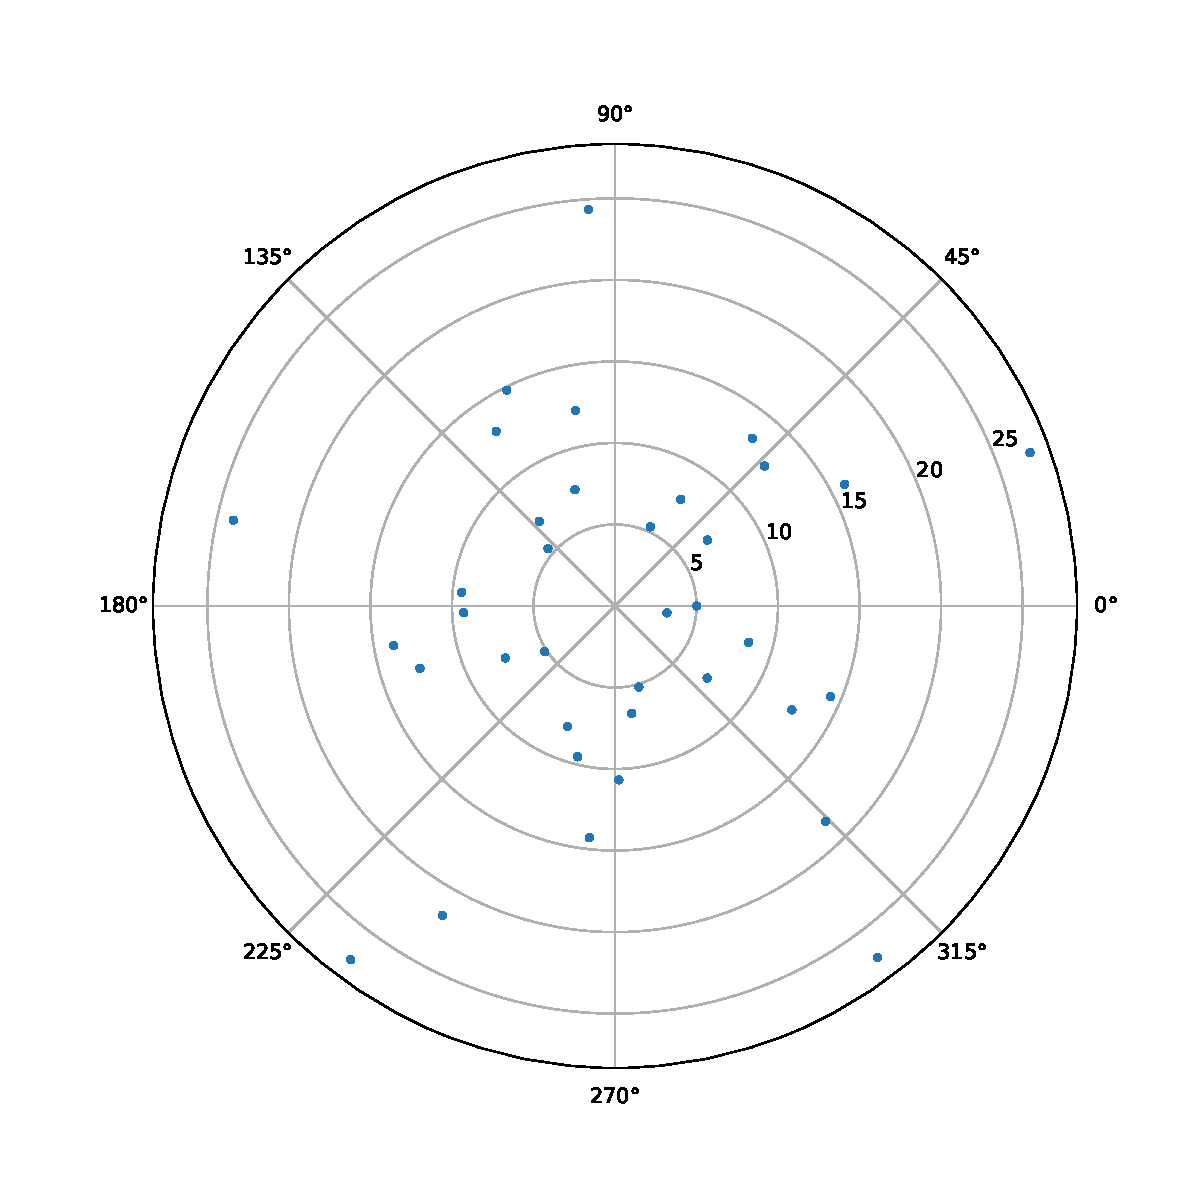
\includegraphics[width=0.8\textwidth]{plots/C_polar4.pdf}
    \caption{Die Winkelverteilung der Amplitude bei der Resonanzfrequenz von \SI{5}{\kilo\hertz}.}
    \label{fig:polar5}
\end{figure}

\begin{figure}
    \centering
    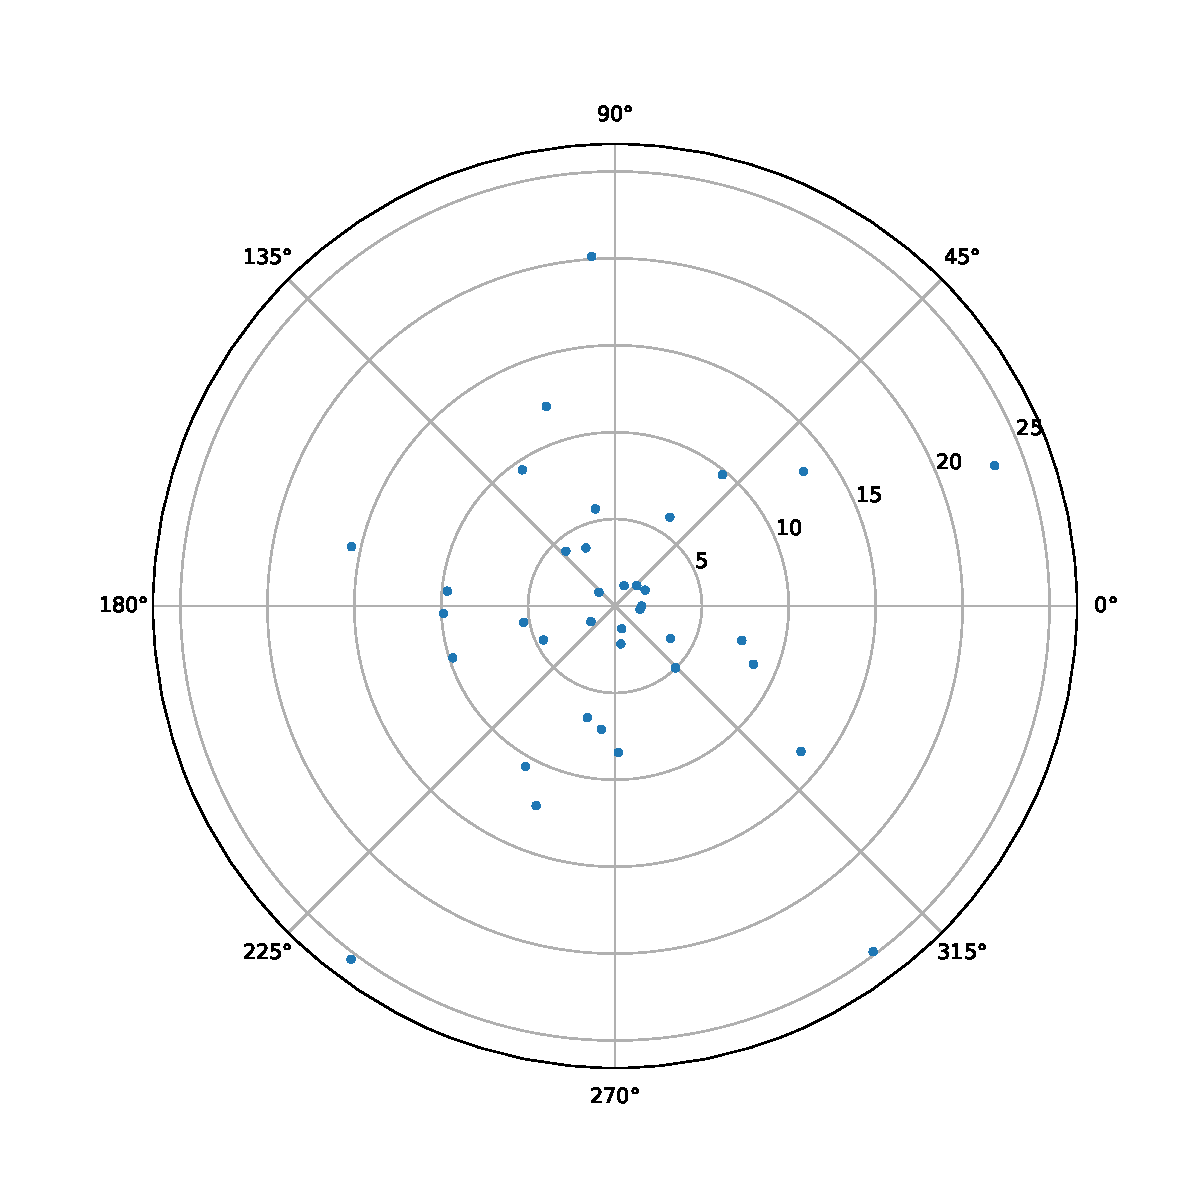
\includegraphics[width=0.8\textwidth]{plots/C_polar3.pdf}
    \caption{Die Winkelverteilung der Amplitude bei der Resonanzfrequenz von \SI{7.4}{\kilo\hertz}.}
    \label{fig:polar74}
\end{figure}


Nur der Peak bei ca. \SI{2.3}{\kilo\hertz} wird mit verschiedenen Zwischenringen überprüft. Die Frequenzspektren des Kugelresonators mit Zwischenringen ist in Abb. \ref{fig:zwischenringe} zu sehen.
Die Aufspaltung des Peaks ist in Abb. \ref{fig:aufspaltung} gegen die Dicke der Ringe aufgetragen.

\begin{figure}
    \centering
    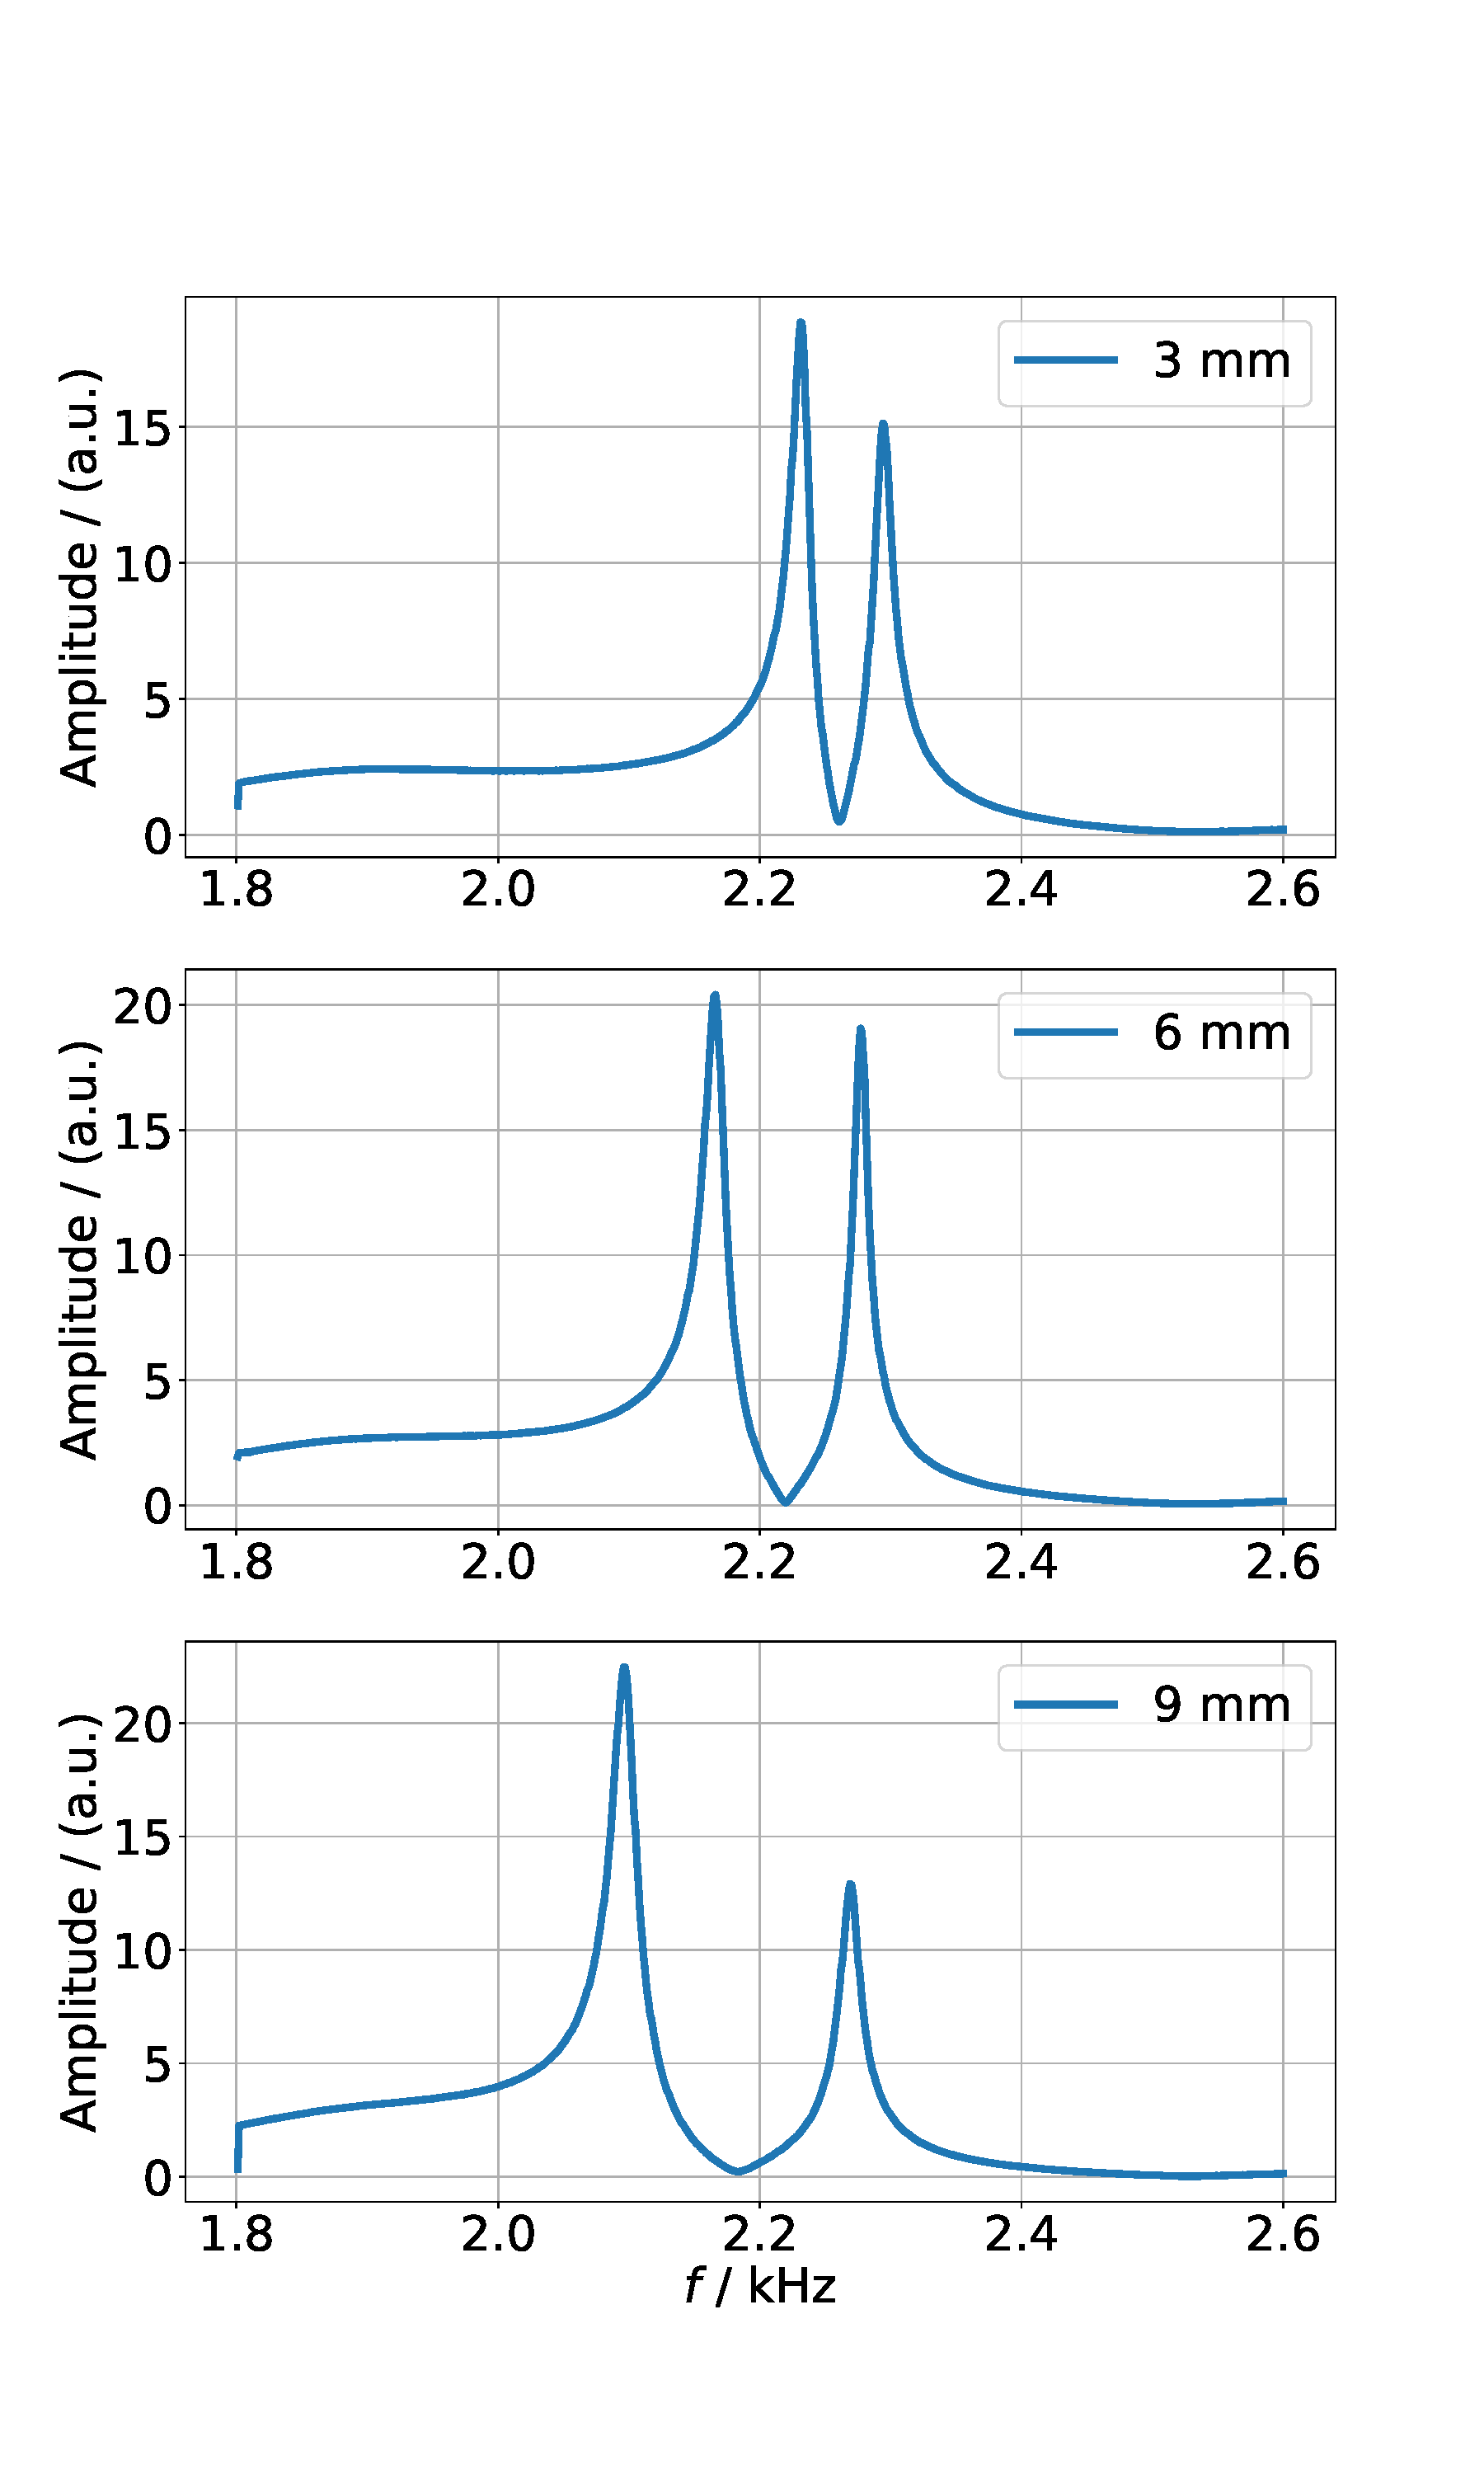
\includegraphics[width=0.8\textwidth]{plots/C_4.pdf}
    \caption{Zu sehen ist das Frequenzspektrum eines Kugelresonators mit Zwischenringen verschiedener Dicke. Oben wurde ein Zwischenring mit \SI{3}{\milli\metre} Dicke verwendet. In der Mitte beträgt die Dicke \SI{6}{\milli\metre} und unten \SI{9}{\milli\metre}}
    \label{fig:zwischenringe}
\end{figure}

\begin{figure}
    \centering
    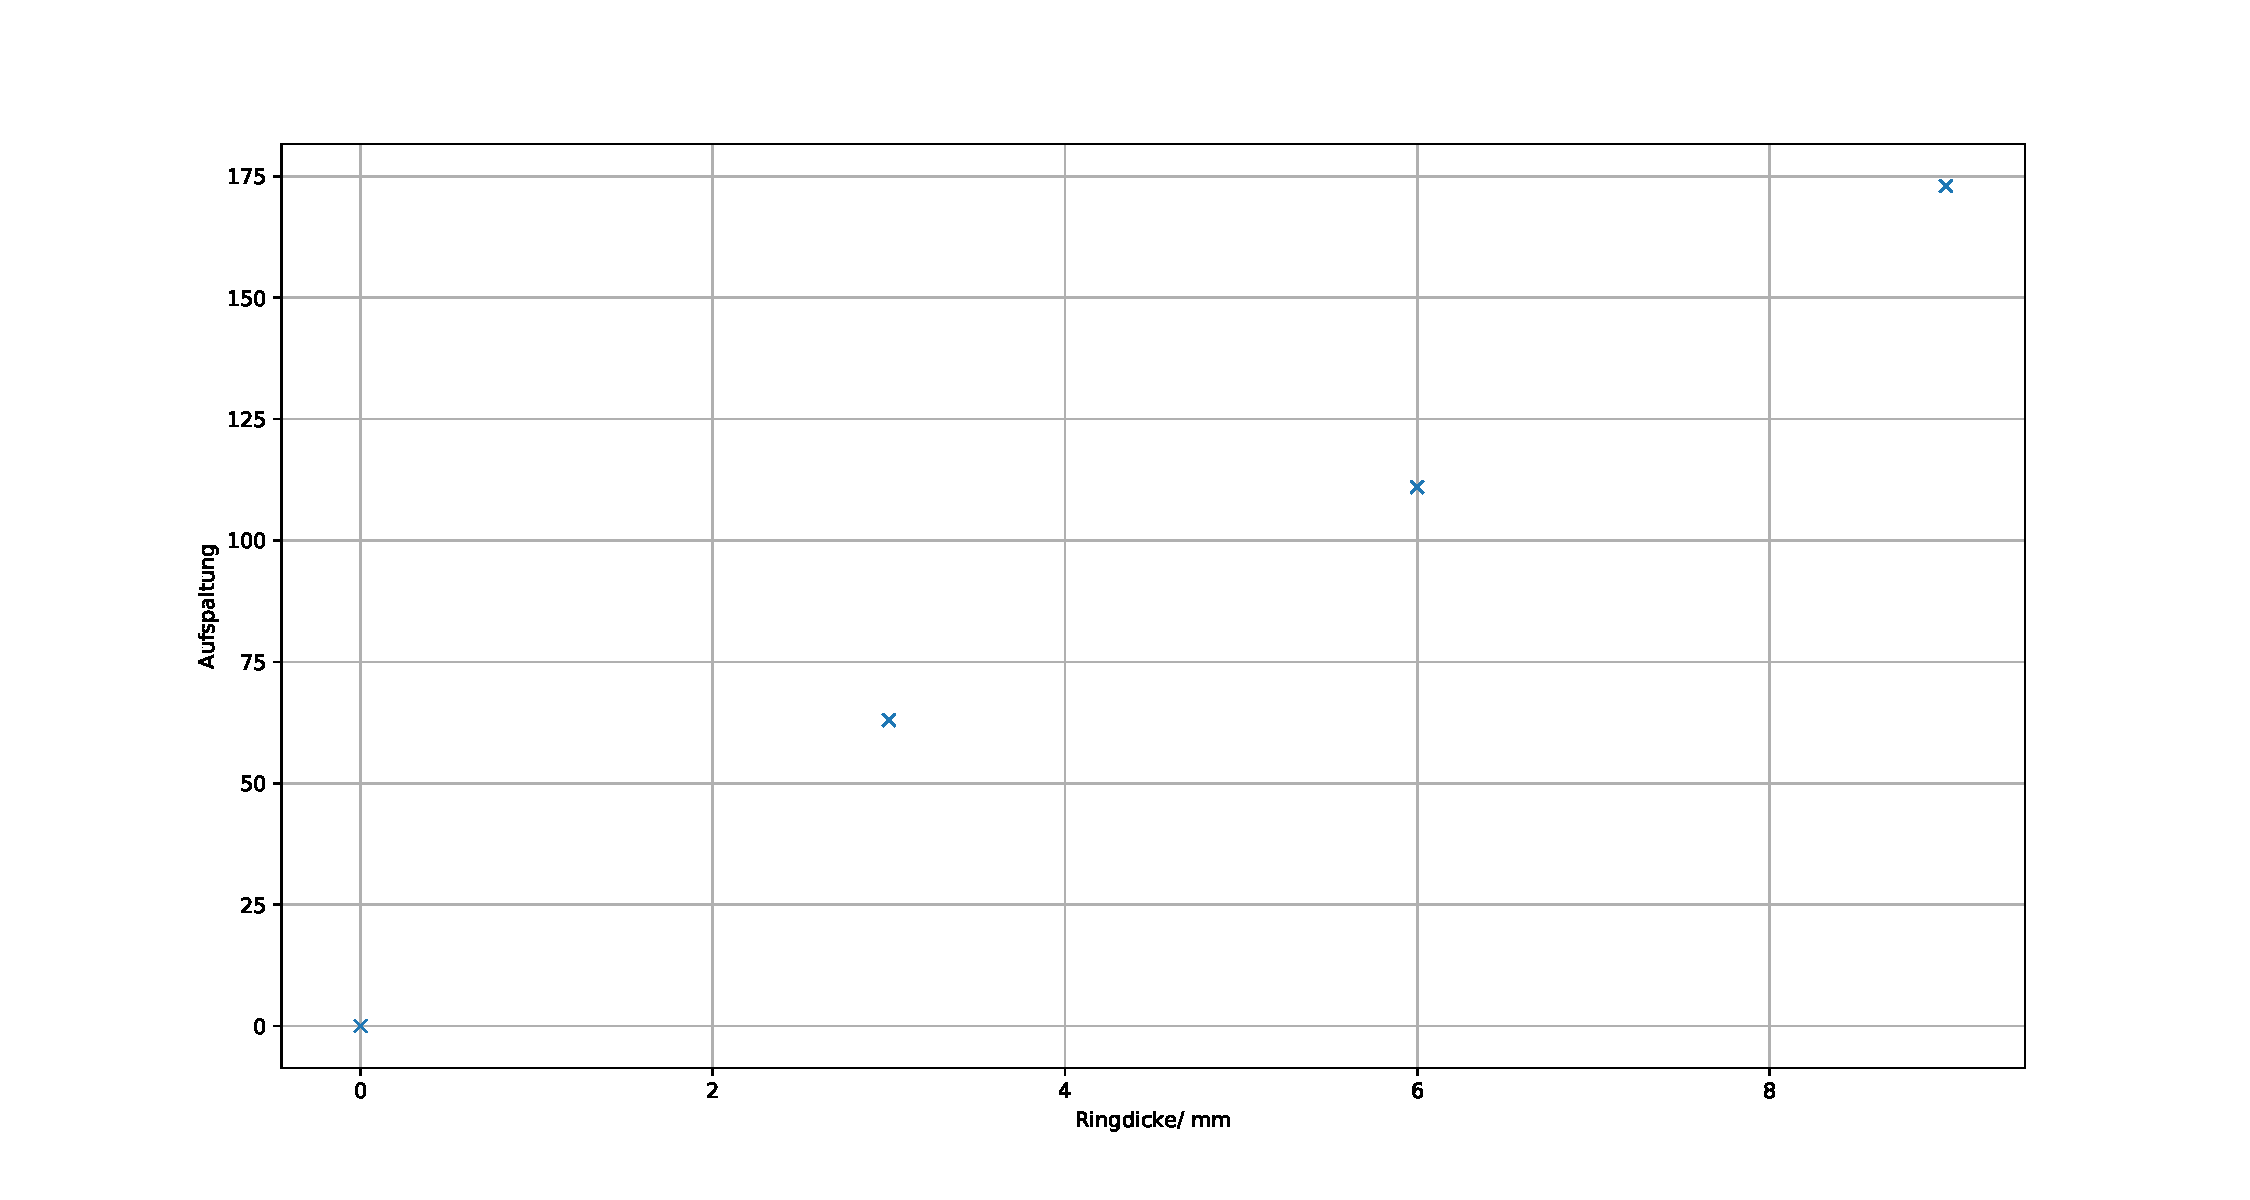
\includegraphics[width=0.8\textwidth]{plots/C_Aufspaltung.pdf}
    \caption{Die Aufspaltung des Peaks ist gegen die Dicke des Zwischenrings aufgetragen. Die einzelnen Datenpunkte sind eingetragen.}
    \label{fig:aufspaltung}
\end{figure}

Mit einer Dicke des Rings von \SI{9}{\milli\meter} wird die Winkelabhängigkeit der Amplitude erneut überprüft.
In Abb. \ref{fig:polar2} ist diese in einem Polarplot aufgetragen. Die dazugehörigen Quantenzahlen sind $l = 0, 1,2,3,4,5$ und $ m = 0, 1, 2,3,4,5$. 

\begin{figure}
    \centering
    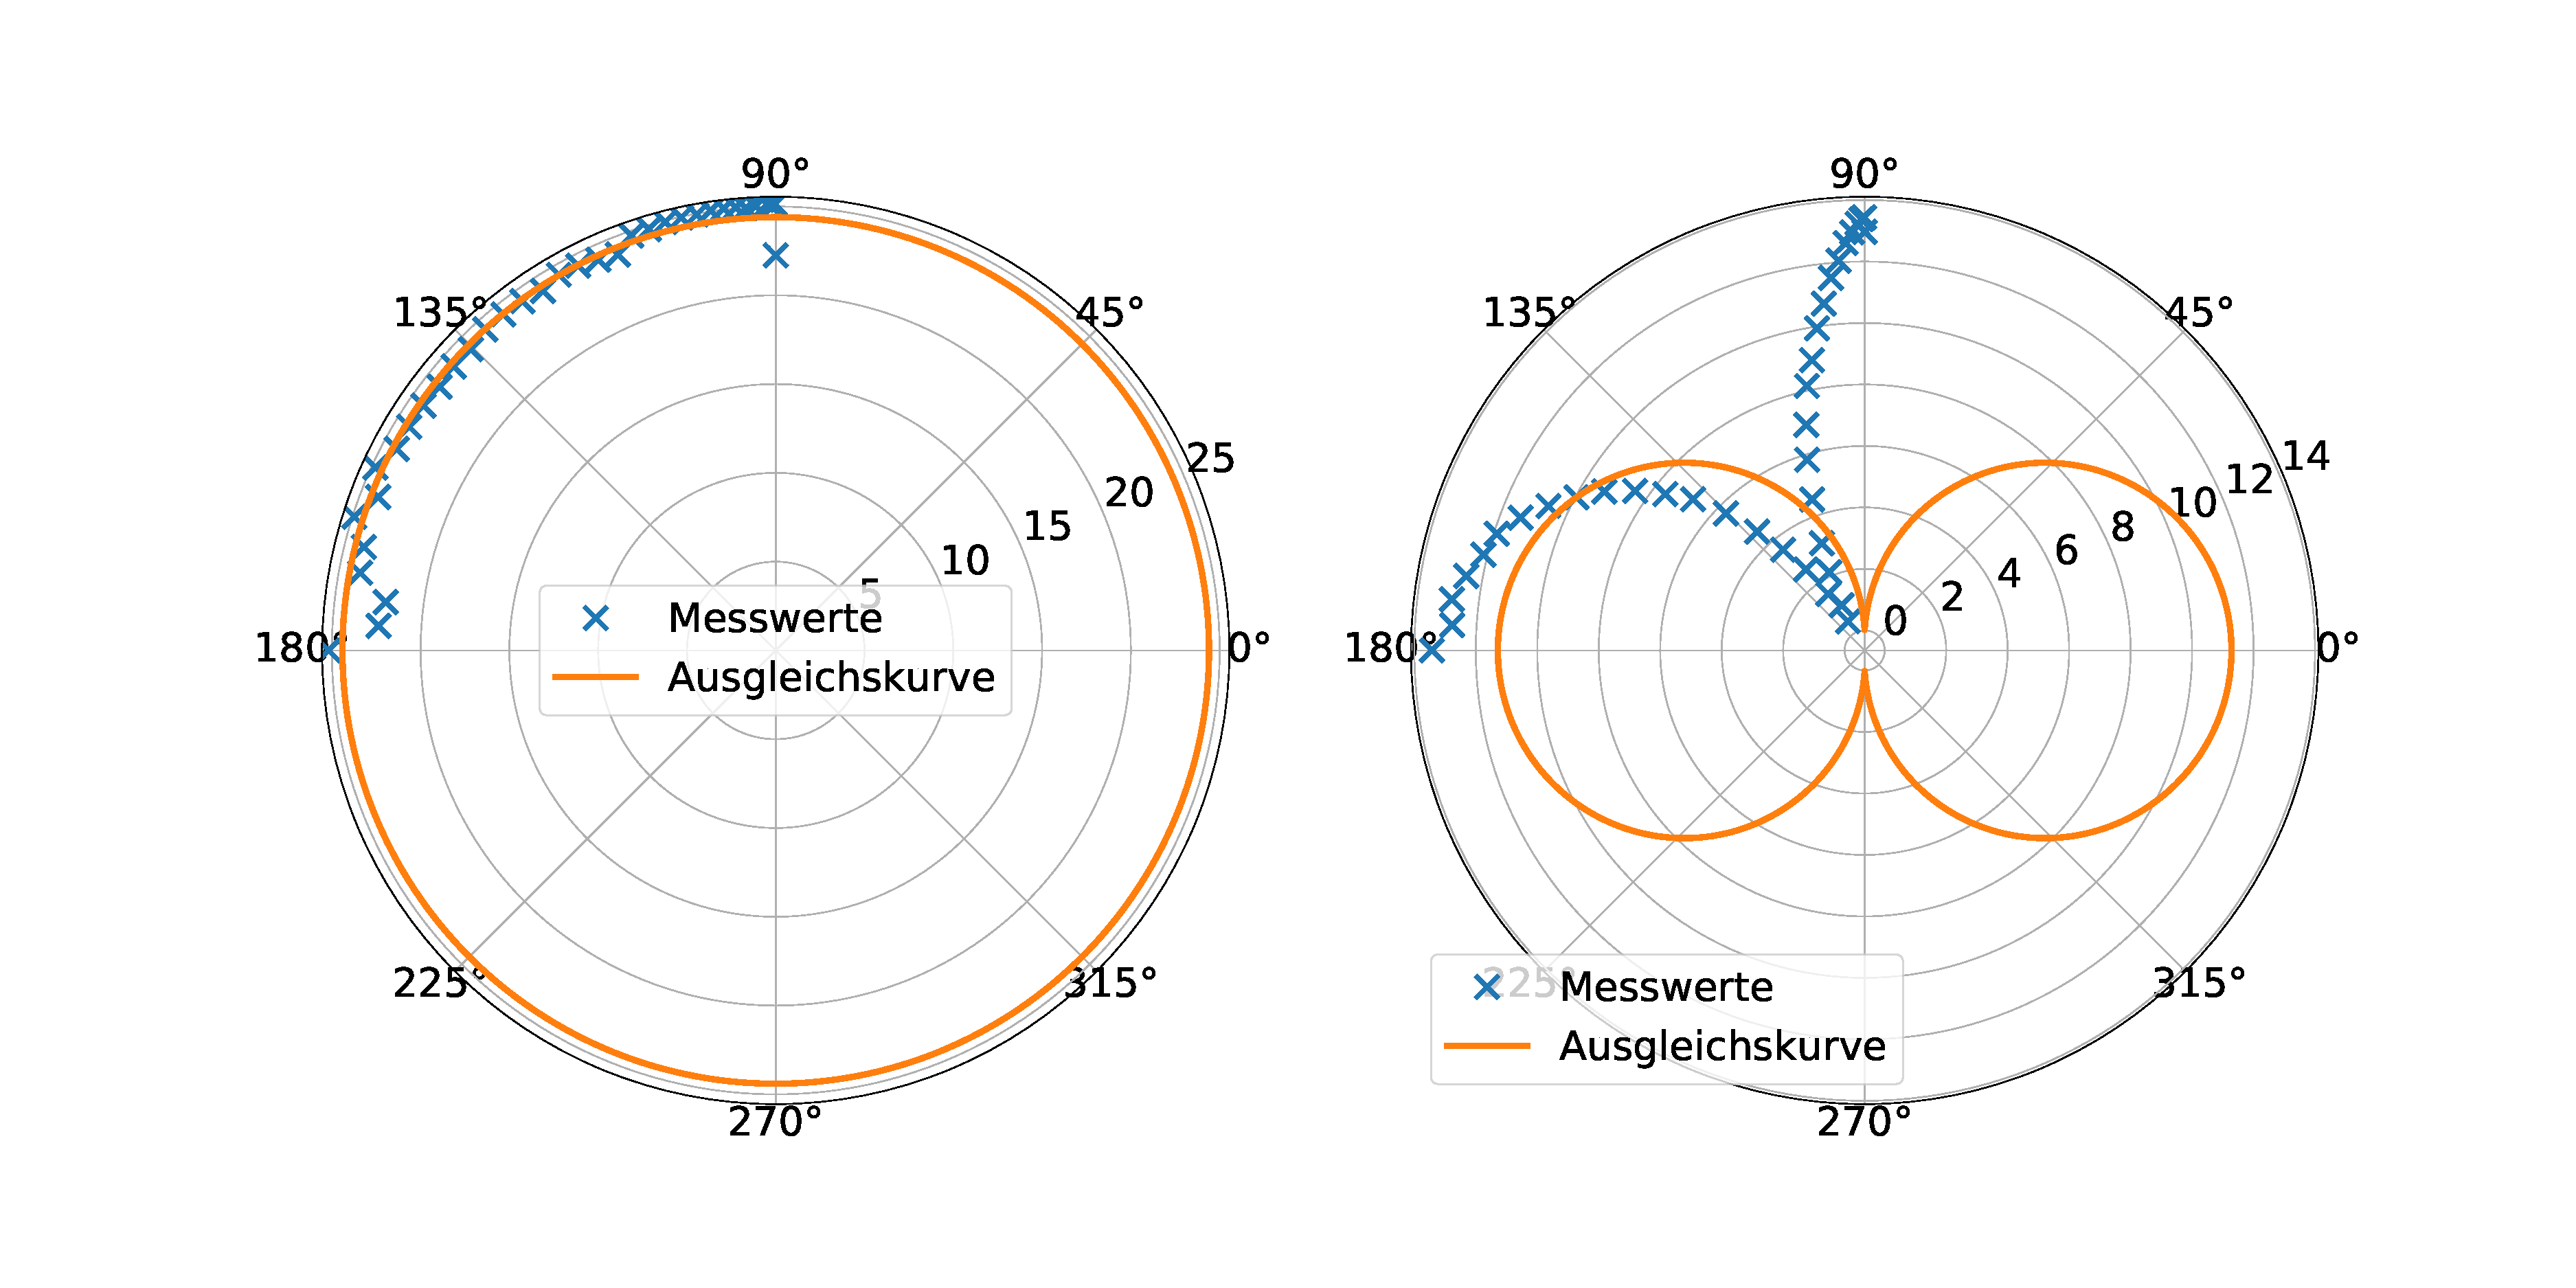
\includegraphics[width=0.8\textwidth]{plots/C_polar5.pdf}
    \caption{Die Winkelverteilung der Amplitude bei der Resonanzfrequenz von \SI{2.3}{\kilo\hertz} mit einem Zwischenring der Dicke \SI{9}{\milli\metre}.}
    \label{fig:polar2}
\end{figure}

\subsection{Wasserstoffmolekül}

Zur Darstellung eines Wasserstoffmoleküls werden zwei Kugelresonatoren, die durch ein Loch verbunden sind, übereinandergesetzt.
Das Frequenzspektrum für den normalen Resonator aus zwei Kugeln und für den Resonator mit Blenden von drei verschiedenen Durchmessern, die zwischen den Kugeln platziert wurden, ist in Abb. \ref{fig:molek1} zu sehen.

\begin{figure}
    \centering
    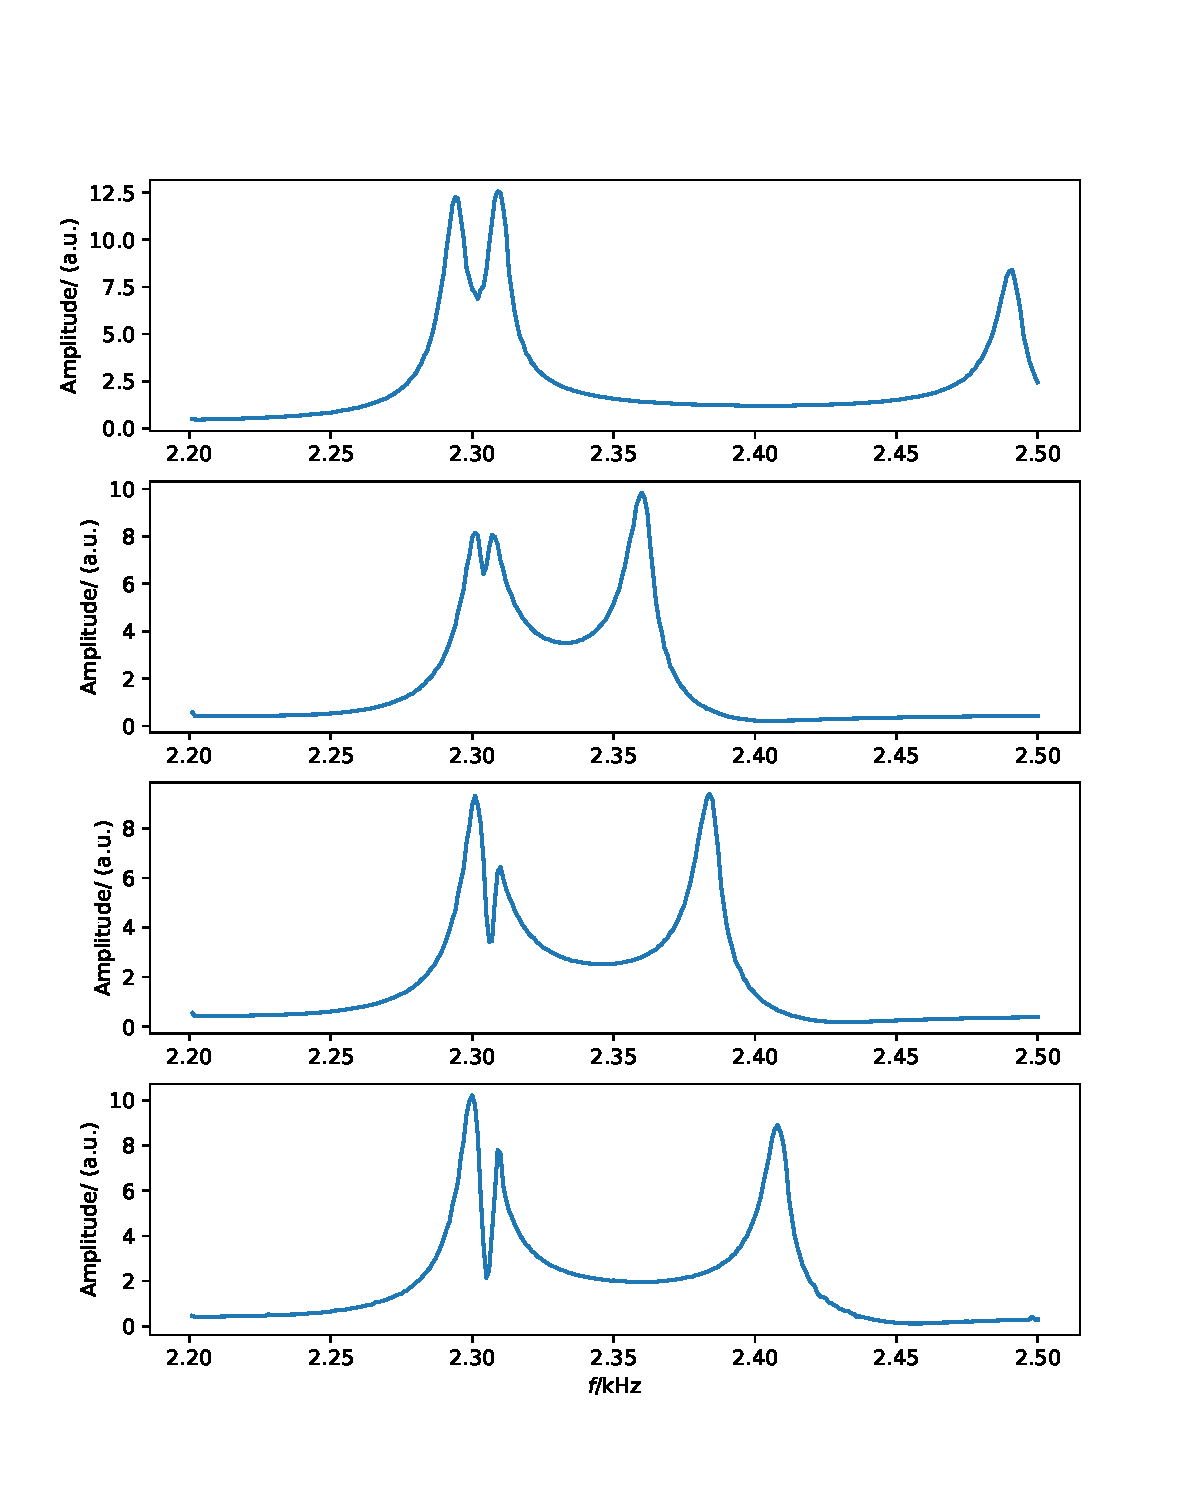
\includegraphics[width=0.8\textwidth]{plots/D_1.pdf}
    \caption{Oben befindet sich das Spektrum für den Resonator ohne Blende. Darunter ist das Spektrum für den Resonator mit einer Blende von \SI{10}{\milli\metre} zu sehen. Darunter ist das Spektrum mit einer Blende von \SI{13}{\milli\metre} und unten das für \SI{16}{\milli\metre}.}
    \label{fig:molek1}
\end{figure}

In Abb. \ref{fig:resonanzen} ist die Resonanzfrequenz in Abhängigkeit vom Blendendurchmesser aufgetragen. Es ist zu beobachten, dass \dots

\begin{figure}
    \centering
    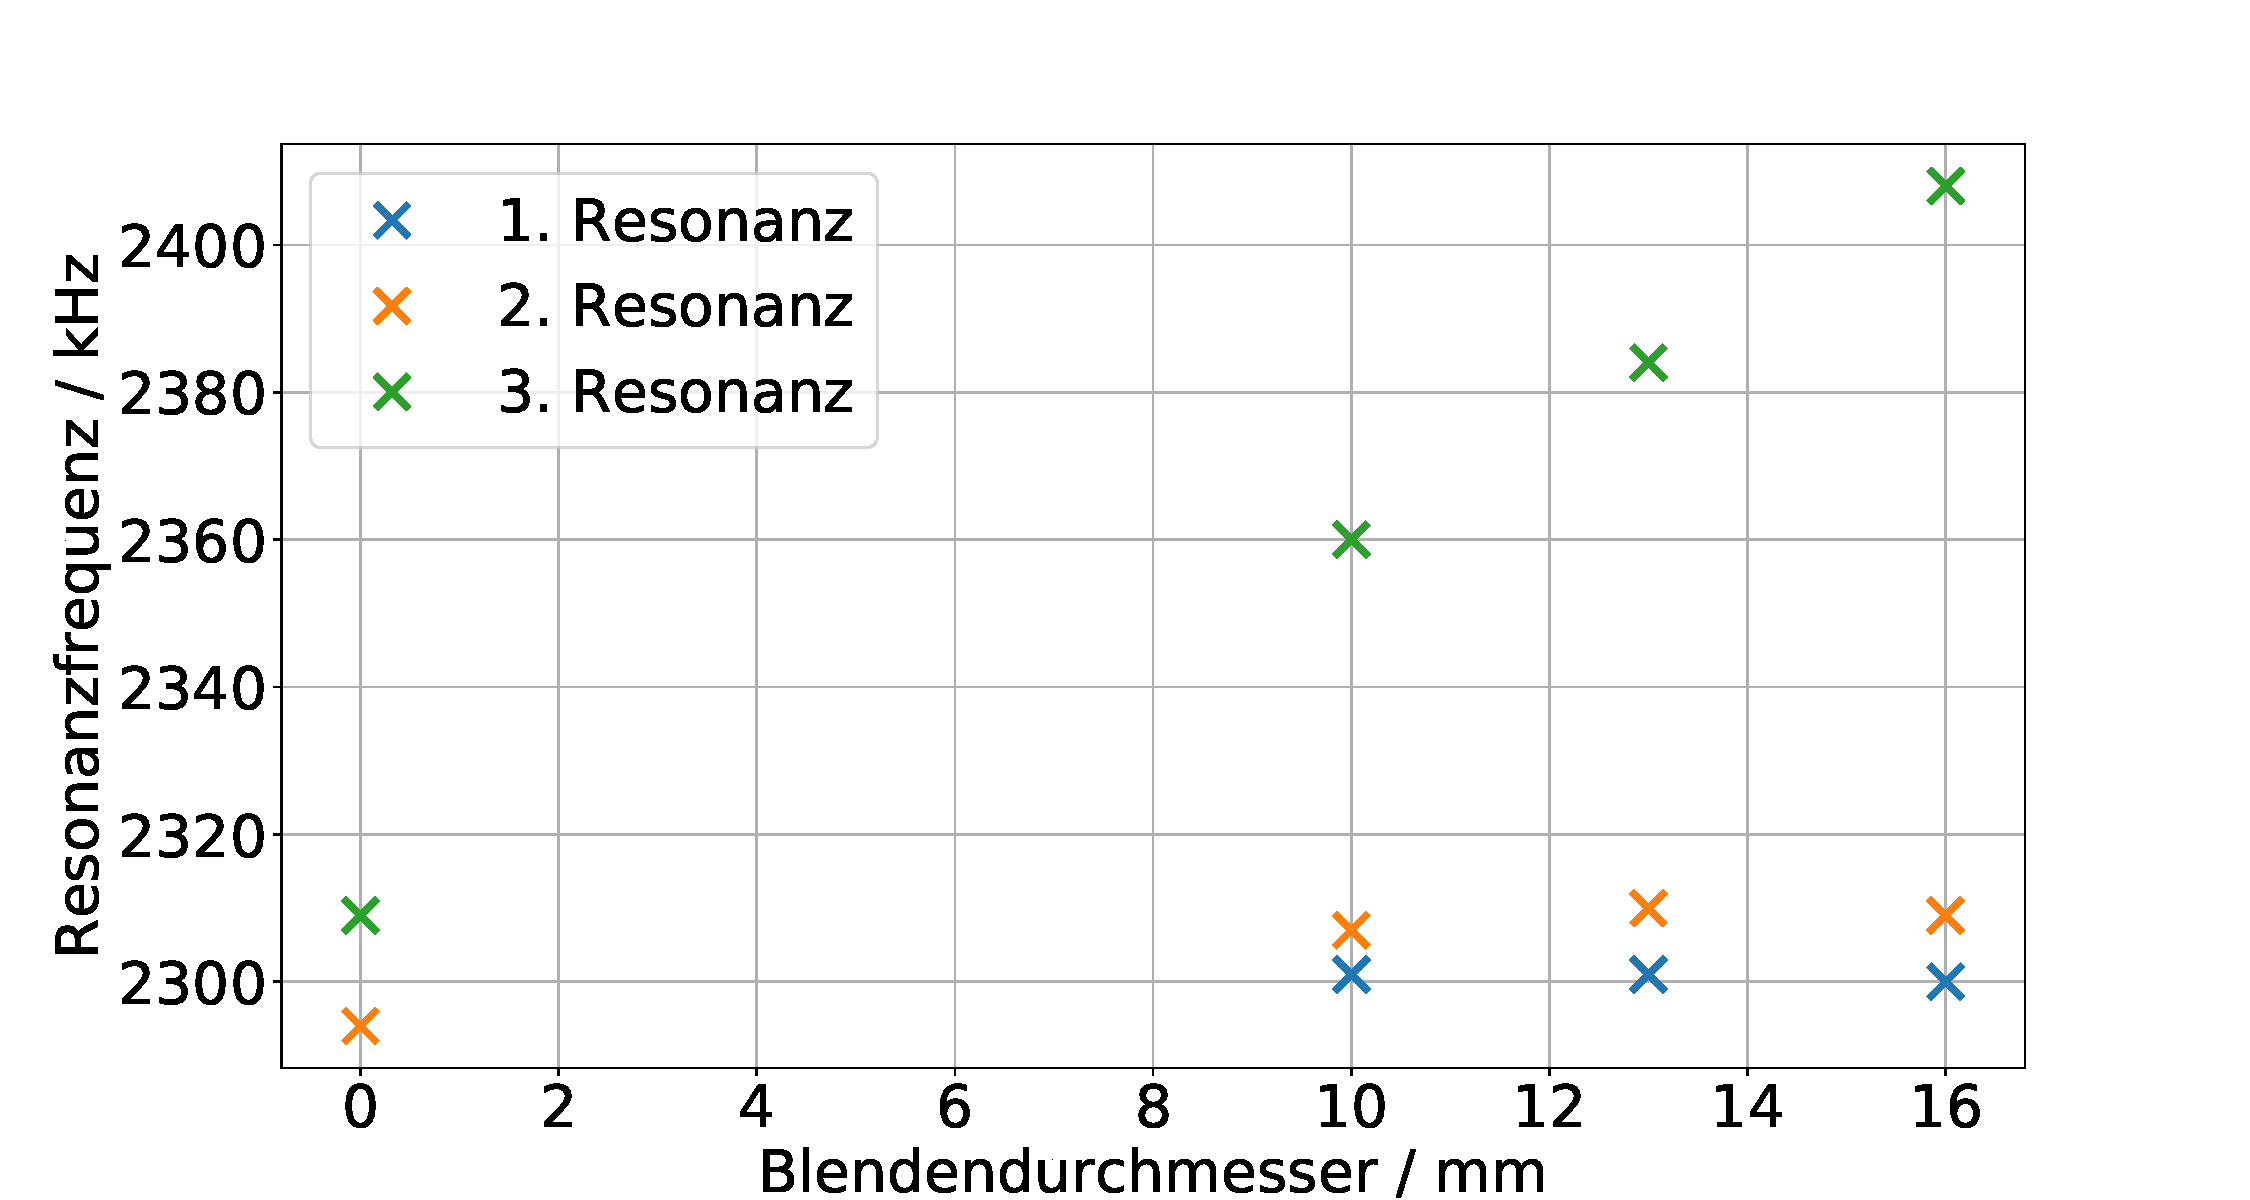
\includegraphics[width=0.8\textwidth]{plots/D_2.pdf}
    \caption{Vorlage}
    \label{fig:resonanzen}
\end{figure}

Das Frequenzspektrum mit einer Blende mit Durchmesser von \SI{16}{\milli\metre} wurde für verschiedene Winkel aufgenommen. Die Winkelverteilung der Amplitude ist in Abb. \ref{fig:polar_molekuel} als Polarplot dargestellt. 

\begin{figure}
    \centering
    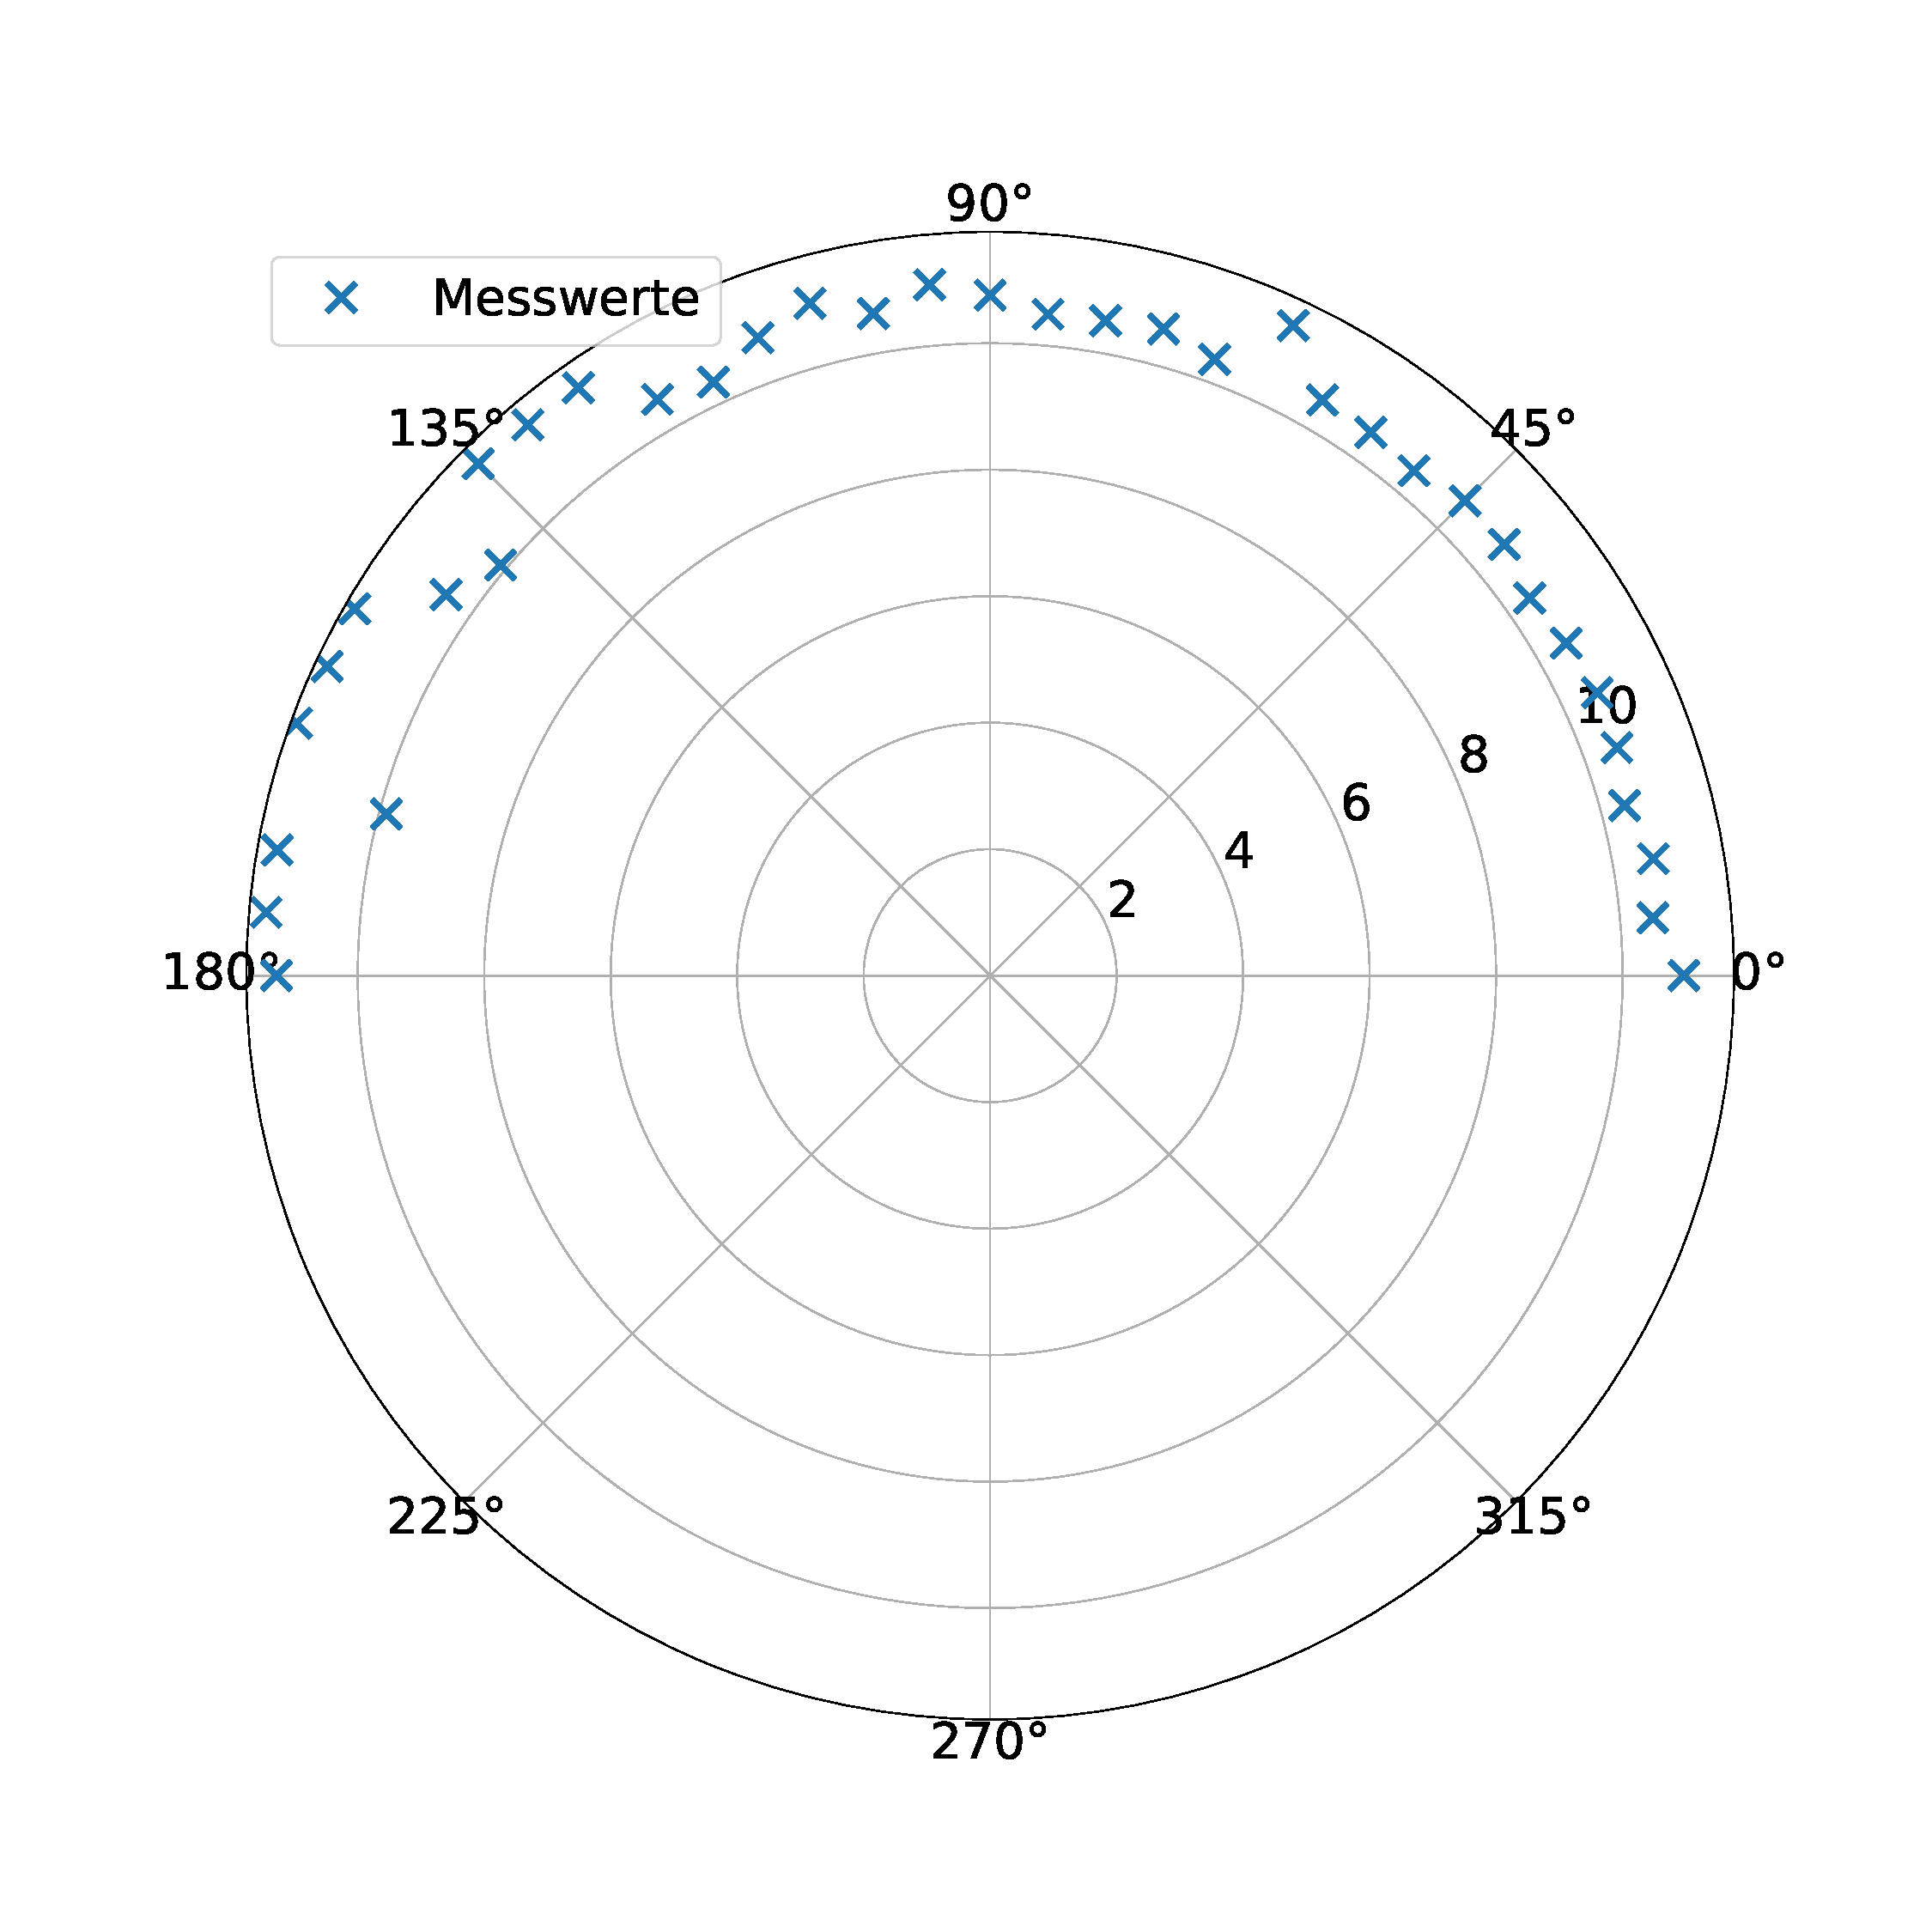
\includegraphics[width=0.8\textwidth]{plots/D_3.pdf}
    \caption{Die Winkelverteilung der Amplitude bei der Resonanzfrequenz von \SI{2.3}{\kilo\hertz} mit einer Blende von \SI{16}{\milli\metre}.}
    \label{fig:polar_molekuel}
\end{figure}

Es wurden die Quantenzustände x,y vermessen. 
Die Phasenverschiebung zwischen der oberen und unteren Kugel wurden bei \SI{180}{\degree} bestimmt. 
Nicht alle vier Peaks sind zu erkennen. Der xy Peak fehlt.